\documentclass[twoside]{book}

% Packages required by doxygen
\usepackage{calc}
\usepackage{doxygen}
\usepackage{graphicx}
\usepackage[utf8]{inputenc}
\usepackage{makeidx}
\usepackage{multicol}
\usepackage{multirow}
\usepackage{textcomp}
\usepackage[table]{xcolor}

% Font selection
\usepackage[T1]{fontenc}
\usepackage{mathptmx}
\usepackage[scaled=.90]{helvet}
\usepackage{courier}
\usepackage{amssymb}
\usepackage{sectsty}
\renewcommand{\familydefault}{\sfdefault}
\allsectionsfont{%
  \fontseries{bc}\selectfont%
  \color{darkgray}%
}
\renewcommand{\DoxyLabelFont}{%
  \fontseries{bc}\selectfont%
  \color{darkgray}%
}

% Page & text layout
\usepackage{geometry}
\geometry{%
  a4paper,%
  top=2.5cm,%
  bottom=2.5cm,%
  left=2.5cm,%
  right=2.5cm%
}
\tolerance=750
\hfuzz=15pt
\hbadness=750
\setlength{\emergencystretch}{15pt}
\setlength{\parindent}{0cm}
\setlength{\parskip}{0.2cm}
\makeatletter
\renewcommand{\paragraph}{%
  \@startsection{paragraph}{4}{0ex}{-1.0ex}{1.0ex}{%
    \normalfont\normalsize\bfseries\SS@parafont%
  }%
}
\renewcommand{\subparagraph}{%
  \@startsection{subparagraph}{5}{0ex}{-1.0ex}{1.0ex}{%
    \normalfont\normalsize\bfseries\SS@subparafont%
  }%
}
\makeatother

% Headers & footers
\usepackage{fancyhdr}
\pagestyle{fancyplain}
\fancyhead[LE]{\fancyplain{}{\bfseries\thepage}}
\fancyhead[CE]{\fancyplain{}{}}
\fancyhead[RE]{\fancyplain{}{\bfseries\leftmark}}
\fancyhead[LO]{\fancyplain{}{\bfseries\rightmark}}
\fancyhead[CO]{\fancyplain{}{}}
\fancyhead[RO]{\fancyplain{}{\bfseries\thepage}}
\fancyfoot[LE]{\fancyplain{}{}}
\fancyfoot[CE]{\fancyplain{}{}}
\fancyfoot[RE]{\fancyplain{}{\bfseries\scriptsize Generated on Tue Nov 29 2016 13\-:51\-:23 for D\-B\-L\-P Query Engine by Doxygen }}
\fancyfoot[LO]{\fancyplain{}{\bfseries\scriptsize Generated on Tue Nov 29 2016 13\-:51\-:23 for D\-B\-L\-P Query Engine by Doxygen }}
\fancyfoot[CO]{\fancyplain{}{}}
\fancyfoot[RO]{\fancyplain{}{}}
\renewcommand{\footrulewidth}{0.4pt}
\renewcommand{\chaptermark}[1]{%
  \markboth{#1}{}%
}
\renewcommand{\sectionmark}[1]{%
  \markright{\thesection\ #1}%
}

% Indices & bibliography
\usepackage{natbib}
\usepackage[titles]{tocloft}
\setcounter{tocdepth}{3}
\setcounter{secnumdepth}{5}
\makeindex

% Hyperlinks (required, but should be loaded last)
\usepackage{ifpdf}
\ifpdf
  \usepackage[pdftex,pagebackref=true]{hyperref}
\else
  \usepackage[ps2pdf,pagebackref=true]{hyperref}
\fi
\hypersetup{%
  colorlinks=true,%
  linkcolor=blue,%
  citecolor=blue,%
  unicode%
}

% Custom commands
\newcommand{\clearemptydoublepage}{%
  \newpage{\pagestyle{empty}\cleardoublepage}%
}


%===== C O N T E N T S =====

\begin{document}

% Titlepage & ToC
\hypersetup{pageanchor=false}
\pagenumbering{roman}
\begin{titlepage}
\vspace*{7cm}
\begin{center}%
{\Large D\-B\-L\-P Query Engine \\[1ex]\large 1.\-0 }\\
\vspace*{1cm}
{\large Generated by Doxygen 1.8.6}\\
\vspace*{0.5cm}
{\small Tue Nov 29 2016 13:51:23}\\
\end{center}
\end{titlepage}
\clearemptydoublepage
\tableofcontents
\clearemptydoublepage
\pagenumbering{arabic}
\hypersetup{pageanchor=true}

%--- Begin generated contents ---
\chapter{Hierarchical Index}
\section{Class Hierarchy}
This inheritance list is sorted roughly, but not completely, alphabetically\-:\begin{DoxyCompactList}
\item \contentsline{section}{Loading}{\pageref{classLoading}}{}
\item \contentsline{section}{Query1\-\_\-\-G\-U\-I}{\pageref{classQuery1__GUI}}{}
\item \contentsline{section}{Query2\-\_\-\-G\-U\-I}{\pageref{classQuery2__GUI}}{}
\item \contentsline{section}{Query3\-\_\-\-G\-U\-I}{\pageref{classQuery3__GUI}}{}
\item Runnable\begin{DoxyCompactList}
\item \contentsline{section}{Xml\-Handler\-Author}{\pageref{classXmlHandlerAuthor}}{}
\item \contentsline{section}{Xml\-Handler\-Title}{\pageref{classXmlHandlerTitle}}{}
\item \contentsline{section}{Xml\-Handler\-Title\-For\-Author}{\pageref{classXmlHandlerTitleForAuthor}}{}
\end{DoxyCompactList}
\item \contentsline{section}{Search}{\pageref{classSearch}}{}
\end{DoxyCompactList}

\chapter{Class Index}
\section{Class List}
Here are the classes, structs, unions and interfaces with brief descriptions\-:\begin{DoxyCompactList}
\item\contentsline{section}{\hyperlink{classLoading}{Loading} }{\pageref{classLoading}}{}
\item\contentsline{section}{\hyperlink{classQuery1__GUI}{Query1\-\_\-\-G\-U\-I} }{\pageref{classQuery1__GUI}}{}
\item\contentsline{section}{\hyperlink{classQuery2__GUI}{Query2\-\_\-\-G\-U\-I} }{\pageref{classQuery2__GUI}}{}
\item\contentsline{section}{\hyperlink{classQuery3__GUI}{Query3\-\_\-\-G\-U\-I} }{\pageref{classQuery3__GUI}}{}
\item\contentsline{section}{\hyperlink{classSearch}{Search} }{\pageref{classSearch}}{}
\item\contentsline{section}{\hyperlink{classXmlHandlerAuthor}{Xml\-Handler\-Author} }{\pageref{classXmlHandlerAuthor}}{}
\item\contentsline{section}{\hyperlink{classXmlHandlerTitle}{Xml\-Handler\-Title} }{\pageref{classXmlHandlerTitle}}{}
\item\contentsline{section}{\hyperlink{classXmlHandlerTitleForAuthor}{Xml\-Handler\-Title\-For\-Author} }{\pageref{classXmlHandlerTitleForAuthor}}{}
\end{DoxyCompactList}

\chapter{File Index}
\section{File List}
Here is a list of all files with brief descriptions\-:\begin{DoxyCompactList}
\item\contentsline{section}{\hyperlink{Loading_8java}{Loading.\-java} }{\pageref{Loading_8java}}{}
\item\contentsline{section}{\hyperlink{Query1__GUI_8java}{Query1\-\_\-\-G\-U\-I.\-java} }{\pageref{Query1__GUI_8java}}{}
\item\contentsline{section}{\hyperlink{Query2__GUI_8java}{Query2\-\_\-\-G\-U\-I.\-java} }{\pageref{Query2__GUI_8java}}{}
\item\contentsline{section}{\hyperlink{Query3__GUI_8java}{Query3\-\_\-\-G\-U\-I.\-java} }{\pageref{Query3__GUI_8java}}{}
\item\contentsline{section}{\hyperlink{Search_8java}{Search.\-java} }{\pageref{Search_8java}}{}
\item\contentsline{section}{\hyperlink{XmlHandler_8java}{Xml\-Handler.\-java} }{\pageref{XmlHandler_8java}}{}
\item\contentsline{section}{\hyperlink{XmlHandlerAuthor_8java}{Xml\-Handler\-Author.\-java} }{\pageref{XmlHandlerAuthor_8java}}{}
\item\contentsline{section}{\hyperlink{XmlHandlerTitle_8java}{Xml\-Handler\-Title.\-java} }{\pageref{XmlHandlerTitle_8java}}{}
\item\contentsline{section}{\hyperlink{XmlHandlerTitleForAuthor_8java}{Xml\-Handler\-Title\-For\-Author.\-java} }{\pageref{XmlHandlerTitleForAuthor_8java}}{}
\end{DoxyCompactList}

\chapter{Class Documentation}
\hypertarget{classLoading}{\section{Loading Class Reference}
\label{classLoading}\index{Loading@{Loading}}
}


Collaboration diagram for Loading\-:
\nopagebreak
\begin{figure}[H]
\begin{center}
\leavevmode
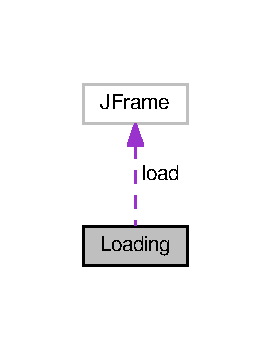
\includegraphics[width=130pt]{classLoading__coll__graph}
\end{center}
\end{figure}
\subsection*{Public Member Functions}
\begin{DoxyCompactItemize}
\item 
\hyperlink{classLoading_a9f9d2da89a7f351415b04901926692b8}{Loading} ()
\item 
void \hyperlink{classLoading_a33fd1d03525ddbdfa8666ad97f390e3d}{start} ()
\item 
void \hyperlink{classLoading_a2b393401cd9bcb3073264ce7f50bc0b4}{stop} ()
\end{DoxyCompactItemize}


\subsection{Detailed Description}


Definition at line 9 of file Loading.\-java.



\subsection{Constructor \& Destructor Documentation}
\hypertarget{classLoading_a9f9d2da89a7f351415b04901926692b8}{\index{Loading@{Loading}!Loading@{Loading}}
\index{Loading@{Loading}!Loading@{Loading}}
\subsubsection[{Loading}]{\setlength{\rightskip}{0pt plus 5cm}Loading.\-Loading (
\begin{DoxyParamCaption}
{}
\end{DoxyParamCaption}
)\hspace{0.3cm}{\ttfamily [inline]}}}\label{classLoading_a9f9d2da89a7f351415b04901926692b8}


Definition at line 11 of file Loading.\-java.


\begin{DoxyCode}
11                     \{
12         load.setSize(300, 100);
13         load.setLocationRelativeTo(null);
14         ImageIcon loading = \textcolor{keyword}{new} ImageIcon(\textcolor{stringliteral}{"ajax-loader.gif"});
15         load.add(\textcolor{keyword}{new} JLabel(loading, JLabel.CENTER));
16         load.setDefaultCloseOperation(JFrame.DO\_NOTHING\_ON\_CLOSE);
17         load.setResizable(\textcolor{keyword}{false});;
18         load.setUndecorated(\textcolor{keyword}{true});
19     \}
\end{DoxyCode}


\subsection{Member Function Documentation}
\hypertarget{classLoading_a33fd1d03525ddbdfa8666ad97f390e3d}{\index{Loading@{Loading}!start@{start}}
\index{start@{start}!Loading@{Loading}}
\subsubsection[{start}]{\setlength{\rightskip}{0pt plus 5cm}void Loading.\-start (
\begin{DoxyParamCaption}
{}
\end{DoxyParamCaption}
)\hspace{0.3cm}{\ttfamily [inline]}}}\label{classLoading_a33fd1d03525ddbdfa8666ad97f390e3d}


Definition at line 20 of file Loading.\-java.


\begin{DoxyCode}
20                        \{
21         load.setVisible(\textcolor{keyword}{true});
22     \}
\end{DoxyCode}
\hypertarget{classLoading_a2b393401cd9bcb3073264ce7f50bc0b4}{\index{Loading@{Loading}!stop@{stop}}
\index{stop@{stop}!Loading@{Loading}}
\subsubsection[{stop}]{\setlength{\rightskip}{0pt plus 5cm}void Loading.\-stop (
\begin{DoxyParamCaption}
{}
\end{DoxyParamCaption}
)\hspace{0.3cm}{\ttfamily [inline]}}}\label{classLoading_a2b393401cd9bcb3073264ce7f50bc0b4}


Definition at line 23 of file Loading.\-java.


\begin{DoxyCode}
23                       \{
24         load.setVisible(\textcolor{keyword}{false});
25     \}
\end{DoxyCode}


The documentation for this class was generated from the following file\-:\begin{DoxyCompactItemize}
\item 
\hyperlink{Loading_8java}{Loading.\-java}\end{DoxyCompactItemize}

\hypertarget{classQuery1__GUI}{\section{Query1\-\_\-\-G\-U\-I Class Reference}
\label{classQuery1__GUI}\index{Query1\-\_\-\-G\-U\-I@{Query1\-\_\-\-G\-U\-I}}
}
\subsection*{Public Member Functions}
\begin{DoxyCompactItemize}
\item 
\hyperlink{classQuery1__GUI_a719f8d96ff9ab4257520f2854a5fdec6}{Query1\-\_\-\-G\-U\-I} (J\-Panel panel)
\item 
void \hyperlink{classQuery1__GUI_a993de0231b4a0748b56c5bb271322c1d}{query1\-\_\-remove} ()
\item 
void \hyperlink{classQuery1__GUI_a84ec3720f7705330af34607bb7f9df97}{query1\-\_\-add} ()
\item 
void \hyperlink{classQuery1__GUI_a296041c237169f0aa259dff727d78c66}{query1\-\_\-search} ()  throws Interrupted\-Exception, I\-O\-Exception
\item 
void \hyperlink{classQuery1__GUI_a4f2a7928d9035191345d523ca6a61474}{query1\-\_\-reset} ()
\end{DoxyCompactItemize}
\subsection*{Public Attributes}
\begin{DoxyCompactItemize}
\item 
int \hyperlink{classQuery1__GUI_aefa26438c30d278901bd04f6f83b57c0}{cache}
\end{DoxyCompactItemize}


\subsection{Detailed Description}


Definition at line 18 of file Query1\-\_\-\-G\-U\-I.\-java.



\subsection{Constructor \& Destructor Documentation}
\hypertarget{classQuery1__GUI_a719f8d96ff9ab4257520f2854a5fdec6}{\index{Query1\-\_\-\-G\-U\-I@{Query1\-\_\-\-G\-U\-I}!Query1\-\_\-\-G\-U\-I@{Query1\-\_\-\-G\-U\-I}}
\index{Query1\-\_\-\-G\-U\-I@{Query1\-\_\-\-G\-U\-I}!Query1_GUI@{Query1\-\_\-\-G\-U\-I}}
\subsubsection[{Query1\-\_\-\-G\-U\-I}]{\setlength{\rightskip}{0pt plus 5cm}Query1\-\_\-\-G\-U\-I.\-Query1\-\_\-\-G\-U\-I (
\begin{DoxyParamCaption}
\item[{J\-Panel}]{panel}
\end{DoxyParamCaption}
)\hspace{0.3cm}{\ttfamily [inline]}}}\label{classQuery1__GUI_a719f8d96ff9ab4257520f2854a5fdec6}


Definition at line 33 of file Query1\-\_\-\-G\-U\-I.\-java.


\begin{DoxyCode}
33                                    \{
34         error.setSize(300, 100);
35         error.setVisible(\textcolor{keyword}{false});
36         error.setLocationRelativeTo(null);
37         error.add(\textcolor{keyword}{new} JLabel(\textcolor{keyword}{new} ImageIcon(\textcolor{stringliteral}{"error.png"}), JLabel.CENTER));
38         query1\_panel.setVisible(\textcolor{keyword}{false});
39         query1\_panel.setBounds(0,125,250,270);
40         drop.setBounds(25,20,200,30);
41         drop.setBackground(Color.white);
42         name.setBounds(30,65,175,30);
43         name.setFont(\textcolor{keyword}{new} Font(\textcolor{stringliteral}{"Courier New"}, Font.PLAIN, 15));
44         text\_name.setBounds(150,65,100,30);
45         year.setBounds(30,100,150,30);
46         year.setFont(\textcolor{keyword}{new} Font(\textcolor{stringliteral}{"Courier New"}, Font.PLAIN, 15));
47         text\_year.setBounds(150,100,100,30);
48         range.setBounds(30,135,175,30);
49         range.setFont(\textcolor{keyword}{new} Font(\textcolor{stringliteral}{"Courier New"}, Font.PLAIN, 15));
50         text\_range1.setBounds(150,135,45,30);
51         text\_range2.setBounds(205,135,45,30);
52         sort\_year.setBounds(20,180,150,20);
53         sort\_relevence.setBounds(20,220,200,20);
54         drop.addItem(\textcolor{stringliteral}{"Search by Author Name"});
55         drop.addItem(\textcolor{stringliteral}{"Search by Title"});
56         buttons.add(sort\_year);
57         sort\_year.setSelected(\textcolor{keyword}{true});
58         buttons.add(sort\_relevence);
59         query1\_panel.add(drop);
60         query1\_panel.add(name);
61         query1\_panel.add(year);
62         query1\_panel.add(range);
63         query1\_panel.add(text\_name);
64         query1\_panel.add(text\_year);
65         query1\_panel.add(text\_range1);
66         query1\_panel.add(text\_range2);
67         query1\_panel.add(sort\_year);
68         query1\_panel.add(sort\_relevence);
69         panel.add(query1\_panel);
70         panel.repaint();
71     \}
\end{DoxyCode}


\subsection{Member Function Documentation}
\hypertarget{classQuery1__GUI_a84ec3720f7705330af34607bb7f9df97}{\index{Query1\-\_\-\-G\-U\-I@{Query1\-\_\-\-G\-U\-I}!query1\-\_\-add@{query1\-\_\-add}}
\index{query1\-\_\-add@{query1\-\_\-add}!Query1_GUI@{Query1\-\_\-\-G\-U\-I}}
\subsubsection[{query1\-\_\-add}]{\setlength{\rightskip}{0pt plus 5cm}void Query1\-\_\-\-G\-U\-I.\-query1\-\_\-add (
\begin{DoxyParamCaption}
{}
\end{DoxyParamCaption}
)\hspace{0.3cm}{\ttfamily [inline]}}}\label{classQuery1__GUI_a84ec3720f7705330af34607bb7f9df97}


Definition at line 75 of file Query1\-\_\-\-G\-U\-I.\-java.


\begin{DoxyCode}
75                             \{
76         query1\_panel.setVisible(\textcolor{keyword}{true});
77     \}
\end{DoxyCode}
\hypertarget{classQuery1__GUI_a993de0231b4a0748b56c5bb271322c1d}{\index{Query1\-\_\-\-G\-U\-I@{Query1\-\_\-\-G\-U\-I}!query1\-\_\-remove@{query1\-\_\-remove}}
\index{query1\-\_\-remove@{query1\-\_\-remove}!Query1_GUI@{Query1\-\_\-\-G\-U\-I}}
\subsubsection[{query1\-\_\-remove}]{\setlength{\rightskip}{0pt plus 5cm}void Query1\-\_\-\-G\-U\-I.\-query1\-\_\-remove (
\begin{DoxyParamCaption}
{}
\end{DoxyParamCaption}
)\hspace{0.3cm}{\ttfamily [inline]}}}\label{classQuery1__GUI_a993de0231b4a0748b56c5bb271322c1d}


Definition at line 72 of file Query1\-\_\-\-G\-U\-I.\-java.


\begin{DoxyCode}
72                                \{
73         query1\_panel.setVisible(\textcolor{keyword}{false});
74     \}
\end{DoxyCode}
\hypertarget{classQuery1__GUI_a4f2a7928d9035191345d523ca6a61474}{\index{Query1\-\_\-\-G\-U\-I@{Query1\-\_\-\-G\-U\-I}!query1\-\_\-reset@{query1\-\_\-reset}}
\index{query1\-\_\-reset@{query1\-\_\-reset}!Query1_GUI@{Query1\-\_\-\-G\-U\-I}}
\subsubsection[{query1\-\_\-reset}]{\setlength{\rightskip}{0pt plus 5cm}void Query1\-\_\-\-G\-U\-I.\-query1\-\_\-reset (
\begin{DoxyParamCaption}
{}
\end{DoxyParamCaption}
)\hspace{0.3cm}{\ttfamily [inline]}}}\label{classQuery1__GUI_a4f2a7928d9035191345d523ca6a61474}


Definition at line 178 of file Query1\-\_\-\-G\-U\-I.\-java.


\begin{DoxyCode}
178                               \{
179         text\_name.setText(\textcolor{stringliteral}{""});
180         text\_range1.setText(\textcolor{stringliteral}{""});
181         text\_range2.setText(\textcolor{stringliteral}{""});
182         text\_year.setText(\textcolor{stringliteral}{""});
183         sort\_year.setSelected(\textcolor{keyword}{true});
184     \}
\end{DoxyCode}
\hypertarget{classQuery1__GUI_a296041c237169f0aa259dff727d78c66}{\index{Query1\-\_\-\-G\-U\-I@{Query1\-\_\-\-G\-U\-I}!query1\-\_\-search@{query1\-\_\-search}}
\index{query1\-\_\-search@{query1\-\_\-search}!Query1_GUI@{Query1\-\_\-\-G\-U\-I}}
\subsubsection[{query1\-\_\-search}]{\setlength{\rightskip}{0pt plus 5cm}void Query1\-\_\-\-G\-U\-I.\-query1\-\_\-search (
\begin{DoxyParamCaption}
{}
\end{DoxyParamCaption}
) throws Interrupted\-Exception, I\-O\-Exception\hspace{0.3cm}{\ttfamily [inline]}}}\label{classQuery1__GUI_a296041c237169f0aa259dff727d78c66}


Definition at line 78 of file Query1\-\_\-\-G\-U\-I.\-java.


\begin{DoxyCode}
78                                                                         \{
79         \textcolor{keywordtype}{int} x;
80         \hyperlink{classQuery1__GUI_aefa26438c30d278901bd04f6f83b57c0}{cache} = 0;
81         \textcolor{keywordflow}{if}(drop.getSelectedItem().equals(\textcolor{stringliteral}{"Search by Author Name"}))\{
82             \textcolor{keywordflow}{if}(!(text\_name.getText().equals(\textcolor{stringliteral}{""})))\{
83                 \textcolor{keywordflow}{if}(!(text\_year.getText().equals(\textcolor{stringliteral}{""}))) x = 2;
84                 \textcolor{keywordflow}{else} \textcolor{keywordflow}{if}(!(text\_range1.getText().equals(\textcolor{stringliteral}{""})) && !(text\_range2.getText().equals(\textcolor{stringliteral}{""})))x = 4;
85                 \textcolor{keywordflow}{else} \textcolor{keywordflow}{if}(sort\_year.isSelected()) x = 1;
86                 \textcolor{keywordflow}{else}\{
87                     x = 0;
88                 \}
89                 \hyperlink{classSearch}{Search} temp = \textcolor{keyword}{new} \hyperlink{classSearch}{Search}(text\_name.getText());
90                 Timer timer = \textcolor{keyword}{new} Timer();
91                 timer.schedule(\textcolor{keyword}{new} TimerTask()\{
92                     @Override
93                     \textcolor{keyword}{public} \textcolor{keywordtype}{void} run() \{
94                         \textcolor{keywordflow}{try} \{
95                             \textcolor{keywordflow}{if}(temp.\hyperlink{classSearch_a02e8edf97002a1cb7a0212339fd9f2df}{working} == 1)\{
96                                 SortSelect(x);
97                                 \hyperlink{classQuery1__GUI_aefa26438c30d278901bd04f6f83b57c0}{cache} = 1;
98                                 timer.cancel();
99                             \}
100                             
101                         \} \textcolor{keywordflow}{catch} (IOException e) \{
102                             e.printStackTrace();
103                         \}
104                 \}\},1000,1000);
105             \}
106             \textcolor{keywordflow}{else}\{
107                 error.setVisible(\textcolor{keyword}{true});
108                 \hyperlink{classQuery1__GUI_aefa26438c30d278901bd04f6f83b57c0}{cache} = 1;
109             \}
110         \}
111         \textcolor{keywordflow}{else} \textcolor{keywordflow}{if}(drop.getSelectedItem().equals(\textcolor{stringliteral}{"Search by Title"}))\{  
112             \textcolor{keywordflow}{if}(!(text\_name.getText().equals(\textcolor{stringliteral}{""})))\{
113                 \textcolor{keywordtype}{int} temp = 4;
114                 \textcolor{keywordflow}{if}(!(text\_year.getText().equals(\textcolor{stringliteral}{""}))) x = 2;
115                 \textcolor{keywordflow}{else} \textcolor{keywordflow}{if}(!(text\_range1.getText().equals(\textcolor{stringliteral}{""})) && !(text\_range2.getText().equals(\textcolor{stringliteral}{""})))x = 4;
116                 \textcolor{keywordflow}{else} \textcolor{keywordflow}{if}(sort\_year.isSelected()) x = 1;
117                 \textcolor{keywordflow}{else} \textcolor{keywordflow}{if}(sort\_relevence.isSelected())\{temp = 0;x=1;\}
118                 \textcolor{keywordflow}{else}\{
119                     x = 0;
120                 \}
121                 \hyperlink{classXmlHandlerTitle}{XmlHandlerTitle} title = \textcolor{keyword}{new} \hyperlink{classXmlHandlerTitle}{XmlHandlerTitle}(text\_name.getText
      (),temp);
122                 Thread t = \textcolor{keyword}{new} Thread(title);
123                 t.start();
124                 Timer timer = \textcolor{keyword}{new} Timer();
125                 timer.schedule(\textcolor{keyword}{new} TimerTask()\{
126                     @Override
127                     \textcolor{keyword}{public} \textcolor{keywordtype}{void} run() \{
128                         \textcolor{keywordflow}{try} \{
129                             \textcolor{keywordflow}{if}(title.\hyperlink{classXmlHandlerTitle_a8430143db4f1036e5db03fbe7e3d451f}{working} == 1)\{
130                                 SortSelect(x);
131                                 \hyperlink{classQuery1__GUI_aefa26438c30d278901bd04f6f83b57c0}{cache} = 1;
132                                 timer.cancel();
133                             \}
134                             
135                         \} \textcolor{keywordflow}{catch} (IOException e) \{
136                             e.printStackTrace();
137                         \}
138                 \}\},1000,1000);
139             \}
140             \textcolor{keywordflow}{else}\{
141                 error.setVisible(\textcolor{keyword}{true});
142                 \hyperlink{classQuery1__GUI_aefa26438c30d278901bd04f6f83b57c0}{cache} = 1;
143             \}
144         \}
145     \}
\end{DoxyCode}


\subsection{Member Data Documentation}
\hypertarget{classQuery1__GUI_aefa26438c30d278901bd04f6f83b57c0}{\index{Query1\-\_\-\-G\-U\-I@{Query1\-\_\-\-G\-U\-I}!cache@{cache}}
\index{cache@{cache}!Query1_GUI@{Query1\-\_\-\-G\-U\-I}}
\subsubsection[{cache}]{\setlength{\rightskip}{0pt plus 5cm}int Query1\-\_\-\-G\-U\-I.\-cache}}\label{classQuery1__GUI_aefa26438c30d278901bd04f6f83b57c0}


Definition at line 32 of file Query1\-\_\-\-G\-U\-I.\-java.



The documentation for this class was generated from the following file\-:\begin{DoxyCompactItemize}
\item 
\hyperlink{Query1__GUI_8java}{Query1\-\_\-\-G\-U\-I.\-java}\end{DoxyCompactItemize}

\hypertarget{classQuery2__GUI}{\section{Query2\-\_\-\-G\-U\-I Class Reference}
\label{classQuery2__GUI}\index{Query2\-\_\-\-G\-U\-I@{Query2\-\_\-\-G\-U\-I}}
}
\subsection*{Public Member Functions}
\begin{DoxyCompactItemize}
\item 
\hyperlink{classQuery2__GUI_af0a78a390c1329af942d0c7c2f870708}{Query2\-\_\-\-G\-U\-I} (J\-Panel panel)
\item 
void \hyperlink{classQuery2__GUI_a59475288434bf7bdbb3c472d46bac1f7}{query2\-\_\-remove} ()
\item 
void \hyperlink{classQuery2__GUI_af8a48da10c813d5fa814647dc205a99f}{query2\-\_\-add} ()
\item 
void \hyperlink{classQuery2__GUI_a7daee1f0408bbc30ff2b520ee1e9bfb4}{query2\-\_\-reset} ()
\end{DoxyCompactItemize}


\subsection{Detailed Description}


Definition at line 6 of file Query2\-\_\-\-G\-U\-I.\-java.



\subsection{Constructor \& Destructor Documentation}
\hypertarget{classQuery2__GUI_af0a78a390c1329af942d0c7c2f870708}{\index{Query2\-\_\-\-G\-U\-I@{Query2\-\_\-\-G\-U\-I}!Query2\-\_\-\-G\-U\-I@{Query2\-\_\-\-G\-U\-I}}
\index{Query2\-\_\-\-G\-U\-I@{Query2\-\_\-\-G\-U\-I}!Query2_GUI@{Query2\-\_\-\-G\-U\-I}}
\subsubsection[{Query2\-\_\-\-G\-U\-I}]{\setlength{\rightskip}{0pt plus 5cm}Query2\-\_\-\-G\-U\-I.\-Query2\-\_\-\-G\-U\-I (
\begin{DoxyParamCaption}
\item[{J\-Panel}]{panel}
\end{DoxyParamCaption}
)\hspace{0.3cm}{\ttfamily [inline]}}}\label{classQuery2__GUI_af0a78a390c1329af942d0c7c2f870708}


Definition at line 10 of file Query2\-\_\-\-G\-U\-I.\-java.


\begin{DoxyCode}
10                                    \{
11         query2\_panel.setVisible(\textcolor{keyword}{false});
12         query2\_panel.setBounds(0,125,250,270);
13         publication.setBounds(30,65,175,30);
14         publication.setFont(\textcolor{keyword}{new} Font(\textcolor{stringliteral}{"Courier New"}, Font.PLAIN, 15));
15         text\_publication.setBounds(170,65,70,30);
16         query2\_panel.add(publication);
17         query2\_panel.add(text\_publication);
18         panel.add(query2\_panel);
19     \}
\end{DoxyCode}


\subsection{Member Function Documentation}
\hypertarget{classQuery2__GUI_af8a48da10c813d5fa814647dc205a99f}{\index{Query2\-\_\-\-G\-U\-I@{Query2\-\_\-\-G\-U\-I}!query2\-\_\-add@{query2\-\_\-add}}
\index{query2\-\_\-add@{query2\-\_\-add}!Query2_GUI@{Query2\-\_\-\-G\-U\-I}}
\subsubsection[{query2\-\_\-add}]{\setlength{\rightskip}{0pt plus 5cm}void Query2\-\_\-\-G\-U\-I.\-query2\-\_\-add (
\begin{DoxyParamCaption}
{}
\end{DoxyParamCaption}
)\hspace{0.3cm}{\ttfamily [inline]}}}\label{classQuery2__GUI_af8a48da10c813d5fa814647dc205a99f}


Definition at line 23 of file Query2\-\_\-\-G\-U\-I.\-java.


\begin{DoxyCode}
23                             \{
24         query2\_panel.setVisible(\textcolor{keyword}{true});
25     \}
\end{DoxyCode}
\hypertarget{classQuery2__GUI_a59475288434bf7bdbb3c472d46bac1f7}{\index{Query2\-\_\-\-G\-U\-I@{Query2\-\_\-\-G\-U\-I}!query2\-\_\-remove@{query2\-\_\-remove}}
\index{query2\-\_\-remove@{query2\-\_\-remove}!Query2_GUI@{Query2\-\_\-\-G\-U\-I}}
\subsubsection[{query2\-\_\-remove}]{\setlength{\rightskip}{0pt plus 5cm}void Query2\-\_\-\-G\-U\-I.\-query2\-\_\-remove (
\begin{DoxyParamCaption}
{}
\end{DoxyParamCaption}
)\hspace{0.3cm}{\ttfamily [inline]}}}\label{classQuery2__GUI_a59475288434bf7bdbb3c472d46bac1f7}


Definition at line 20 of file Query2\-\_\-\-G\-U\-I.\-java.


\begin{DoxyCode}
20                                \{
21         query2\_panel.setVisible(\textcolor{keyword}{false});
22     \}
\end{DoxyCode}
\hypertarget{classQuery2__GUI_a7daee1f0408bbc30ff2b520ee1e9bfb4}{\index{Query2\-\_\-\-G\-U\-I@{Query2\-\_\-\-G\-U\-I}!query2\-\_\-reset@{query2\-\_\-reset}}
\index{query2\-\_\-reset@{query2\-\_\-reset}!Query2_GUI@{Query2\-\_\-\-G\-U\-I}}
\subsubsection[{query2\-\_\-reset}]{\setlength{\rightskip}{0pt plus 5cm}void Query2\-\_\-\-G\-U\-I.\-query2\-\_\-reset (
\begin{DoxyParamCaption}
{}
\end{DoxyParamCaption}
)\hspace{0.3cm}{\ttfamily [inline]}}}\label{classQuery2__GUI_a7daee1f0408bbc30ff2b520ee1e9bfb4}


Definition at line 26 of file Query2\-\_\-\-G\-U\-I.\-java.


\begin{DoxyCode}
26                               \{
27         text\_publication.setText(\textcolor{stringliteral}{""});
28     \}
\end{DoxyCode}


The documentation for this class was generated from the following file\-:\begin{DoxyCompactItemize}
\item 
\hyperlink{Query2__GUI_8java}{Query2\-\_\-\-G\-U\-I.\-java}\end{DoxyCompactItemize}

\hypertarget{classQuery3__GUI}{\section{Query3\-\_\-\-G\-U\-I Class Reference}
\label{classQuery3__GUI}\index{Query3\-\_\-\-G\-U\-I@{Query3\-\_\-\-G\-U\-I}}
}
\subsection*{Public Member Functions}
\begin{DoxyCompactItemize}
\item 
\hyperlink{classQuery3__GUI_a56170789543e9d2ed2b254d8b4bfb72c}{Query3\-\_\-\-G\-U\-I} (J\-Panel panel)
\item 
void \hyperlink{classQuery3__GUI_a63b8b44746b31e14d0c287fb7cf5a407}{query3\-\_\-remove} ()
\item 
void \hyperlink{classQuery3__GUI_a62d42f02d00a389220b3d837fe8fb914}{query3\-\_\-add} ()
\item 
void \hyperlink{classQuery3__GUI_ae28882c0291a82d66578cd8cbef24dcf}{query3\-\_\-reset} ()
\item 
double\mbox{[}$\,$\mbox{]} \hyperlink{classQuery3__GUI_a672b09c39e9d93a5ead04f254d160074}{holt\-\_\-alg} (double h, double y\-\_\-last, double y\-\_\-pred, double T\-\_\-pred, double alpha, double beta)
\item 
Array\-List$<$ Double $>$ \hyperlink{classQuery3__GUI_a5a3482ed71d3e567e47607ddb61028cc}{smoothing} (double\mbox{[}$\,$\mbox{]} t, double\mbox{[}$\,$\mbox{]} y, double alpha, double beta)
\end{DoxyCompactItemize}


\subsection{Detailed Description}


Definition at line 8 of file Query3\-\_\-\-G\-U\-I.\-java.



\subsection{Constructor \& Destructor Documentation}
\hypertarget{classQuery3__GUI_a56170789543e9d2ed2b254d8b4bfb72c}{\index{Query3\-\_\-\-G\-U\-I@{Query3\-\_\-\-G\-U\-I}!Query3\-\_\-\-G\-U\-I@{Query3\-\_\-\-G\-U\-I}}
\index{Query3\-\_\-\-G\-U\-I@{Query3\-\_\-\-G\-U\-I}!Query3_GUI@{Query3\-\_\-\-G\-U\-I}}
\subsubsection[{Query3\-\_\-\-G\-U\-I}]{\setlength{\rightskip}{0pt plus 5cm}Query3\-\_\-\-G\-U\-I.\-Query3\-\_\-\-G\-U\-I (
\begin{DoxyParamCaption}
\item[{J\-Panel}]{panel}
\end{DoxyParamCaption}
)\hspace{0.3cm}{\ttfamily [inline]}}}\label{classQuery3__GUI_a56170789543e9d2ed2b254d8b4bfb72c}


Definition at line 14 of file Query3\-\_\-\-G\-U\-I.\-java.


\begin{DoxyCode}
14                                    \{
15         query3\_panel.setVisible(\textcolor{keyword}{false});
16         query3\_panel.setBounds(0,125,250,270);
17         name.setBounds(30,65,175,30);
18         year.setBounds(30,100,175,30);
19         name.setFont(\textcolor{keyword}{new} Font(\textcolor{stringliteral}{"Courier New"}, Font.PLAIN, 15));
20         year.setFont(\textcolor{keyword}{new} Font(\textcolor{stringliteral}{"Courier New"}, Font.PLAIN, 15));
21         text\_name.setBounds(140,65,100,30);
22         text\_year.setBounds(170,100,70,30);
23         query3\_panel.add(name);
24         query3\_panel.add(year);
25         query3\_panel.add(text\_name);
26         query3\_panel.add(text\_year);
27         panel.add(query3\_panel);
28     \}
\end{DoxyCode}


\subsection{Member Function Documentation}
\hypertarget{classQuery3__GUI_a672b09c39e9d93a5ead04f254d160074}{\index{Query3\-\_\-\-G\-U\-I@{Query3\-\_\-\-G\-U\-I}!holt\-\_\-alg@{holt\-\_\-alg}}
\index{holt\-\_\-alg@{holt\-\_\-alg}!Query3_GUI@{Query3\-\_\-\-G\-U\-I}}
\subsubsection[{holt\-\_\-alg}]{\setlength{\rightskip}{0pt plus 5cm}double \mbox{[}$\,$\mbox{]} Query3\-\_\-\-G\-U\-I.\-holt\-\_\-alg (
\begin{DoxyParamCaption}
\item[{double}]{h, }
\item[{double}]{y\-\_\-last, }
\item[{double}]{y\-\_\-pred, }
\item[{double}]{T\-\_\-pred, }
\item[{double}]{alpha, }
\item[{double}]{beta}
\end{DoxyParamCaption}
)\hspace{0.3cm}{\ttfamily [inline]}}}\label{classQuery3__GUI_a672b09c39e9d93a5ead04f254d160074}


Definition at line 39 of file Query3\-\_\-\-G\-U\-I.\-java.


\begin{DoxyCode}
39                                                                                                          \{
40         \textcolor{keywordtype}{double} pred\_y\_new = alpha * y\_last + (1-alpha) * (y\_pred + T\_pred * h);
41         \textcolor{keywordtype}{double} pred\_t\_new = beta * (pred\_y\_new - y\_pred)/h + (1-beta)*T\_pred;
42         \textcolor{keywordtype}{double} [] temp = \textcolor{keyword}{new} \textcolor{keywordtype}{double}[2];
43         temp[0] = pred\_y\_new;
44         temp[1] = pred\_t\_new;
45         \textcolor{keywordflow}{return} temp;
46     \}
\end{DoxyCode}
\hypertarget{classQuery3__GUI_a62d42f02d00a389220b3d837fe8fb914}{\index{Query3\-\_\-\-G\-U\-I@{Query3\-\_\-\-G\-U\-I}!query3\-\_\-add@{query3\-\_\-add}}
\index{query3\-\_\-add@{query3\-\_\-add}!Query3_GUI@{Query3\-\_\-\-G\-U\-I}}
\subsubsection[{query3\-\_\-add}]{\setlength{\rightskip}{0pt plus 5cm}void Query3\-\_\-\-G\-U\-I.\-query3\-\_\-add (
\begin{DoxyParamCaption}
{}
\end{DoxyParamCaption}
)\hspace{0.3cm}{\ttfamily [inline]}}}\label{classQuery3__GUI_a62d42f02d00a389220b3d837fe8fb914}


Definition at line 32 of file Query3\-\_\-\-G\-U\-I.\-java.


\begin{DoxyCode}
32                             \{
33         query3\_panel.setVisible(\textcolor{keyword}{true});
34     \}
\end{DoxyCode}
\hypertarget{classQuery3__GUI_a63b8b44746b31e14d0c287fb7cf5a407}{\index{Query3\-\_\-\-G\-U\-I@{Query3\-\_\-\-G\-U\-I}!query3\-\_\-remove@{query3\-\_\-remove}}
\index{query3\-\_\-remove@{query3\-\_\-remove}!Query3_GUI@{Query3\-\_\-\-G\-U\-I}}
\subsubsection[{query3\-\_\-remove}]{\setlength{\rightskip}{0pt plus 5cm}void Query3\-\_\-\-G\-U\-I.\-query3\-\_\-remove (
\begin{DoxyParamCaption}
{}
\end{DoxyParamCaption}
)\hspace{0.3cm}{\ttfamily [inline]}}}\label{classQuery3__GUI_a63b8b44746b31e14d0c287fb7cf5a407}


Definition at line 29 of file Query3\-\_\-\-G\-U\-I.\-java.


\begin{DoxyCode}
29                                \{
30         query3\_panel.setVisible(\textcolor{keyword}{false});
31     \}
\end{DoxyCode}
\hypertarget{classQuery3__GUI_ae28882c0291a82d66578cd8cbef24dcf}{\index{Query3\-\_\-\-G\-U\-I@{Query3\-\_\-\-G\-U\-I}!query3\-\_\-reset@{query3\-\_\-reset}}
\index{query3\-\_\-reset@{query3\-\_\-reset}!Query3_GUI@{Query3\-\_\-\-G\-U\-I}}
\subsubsection[{query3\-\_\-reset}]{\setlength{\rightskip}{0pt plus 5cm}void Query3\-\_\-\-G\-U\-I.\-query3\-\_\-reset (
\begin{DoxyParamCaption}
{}
\end{DoxyParamCaption}
)\hspace{0.3cm}{\ttfamily [inline]}}}\label{classQuery3__GUI_ae28882c0291a82d66578cd8cbef24dcf}


Definition at line 35 of file Query3\-\_\-\-G\-U\-I.\-java.


\begin{DoxyCode}
35                               \{
36         text\_name.setText(\textcolor{stringliteral}{""});
37         text\_year.setText(\textcolor{stringliteral}{""});
38     \}
\end{DoxyCode}
\hypertarget{classQuery3__GUI_a5a3482ed71d3e567e47607ddb61028cc}{\index{Query3\-\_\-\-G\-U\-I@{Query3\-\_\-\-G\-U\-I}!smoothing@{smoothing}}
\index{smoothing@{smoothing}!Query3_GUI@{Query3\-\_\-\-G\-U\-I}}
\subsubsection[{smoothing}]{\setlength{\rightskip}{0pt plus 5cm}Array\-List$<$Double$>$ Query3\-\_\-\-G\-U\-I.\-smoothing (
\begin{DoxyParamCaption}
\item[{double\mbox{[}$\,$\mbox{]}}]{t, }
\item[{double\mbox{[}$\,$\mbox{]}}]{y, }
\item[{double}]{alpha, }
\item[{double}]{beta}
\end{DoxyParamCaption}
)\hspace{0.3cm}{\ttfamily [inline]}}}\label{classQuery3__GUI_a5a3482ed71d3e567e47607ddb61028cc}


Definition at line 47 of file Query3\-\_\-\-G\-U\-I.\-java.


\begin{DoxyCode}
47                                                                                       \{
48         \textcolor{keywordtype}{double} pred\_y = y[1];
49         \textcolor{keywordtype}{double} pred\_t = (y[1] - y[0])/(t[1] - t[0]);
50         ArrayList<Double> y\_hat = \textcolor{keyword}{new} ArrayList<Double>();
51         y\_hat.add(y[0]);
52         y\_hat.add(y[1]);
53         \textcolor{keywordflow}{return} y\_hat;
54         
55     \}
\end{DoxyCode}


The documentation for this class was generated from the following file\-:\begin{DoxyCompactItemize}
\item 
\hyperlink{Query3__GUI_8java}{Query3\-\_\-\-G\-U\-I.\-java}\end{DoxyCompactItemize}

\hypertarget{classSearch}{\section{Search Class Reference}
\label{classSearch}\index{Search@{Search}}
}
\subsection*{Public Member Functions}
\begin{DoxyCompactItemize}
\item 
\hyperlink{classSearch_a44bd8a4b037953a006bf82ec075b16bd}{Search} (String x)  throws Interrupted\-Exception, I\-O\-Exception
\end{DoxyCompactItemize}
\subsection*{Public Attributes}
\begin{DoxyCompactItemize}
\item 
volatile int \hyperlink{classSearch_a02e8edf97002a1cb7a0212339fd9f2df}{working}
\end{DoxyCompactItemize}


\subsection{Detailed Description}


Definition at line 10 of file Search.\-java.



\subsection{Constructor \& Destructor Documentation}
\hypertarget{classSearch_a44bd8a4b037953a006bf82ec075b16bd}{\index{Search@{Search}!Search@{Search}}
\index{Search@{Search}!Search@{Search}}
\subsubsection[{Search}]{\setlength{\rightskip}{0pt plus 5cm}Search.\-Search (
\begin{DoxyParamCaption}
\item[{String}]{x}
\end{DoxyParamCaption}
) throws Interrupted\-Exception, I\-O\-Exception\hspace{0.3cm}{\ttfamily [inline]}}}\label{classSearch_a44bd8a4b037953a006bf82ec075b16bd}


Definition at line 13 of file Search.\-java.


\begin{DoxyCode}
13                                                                     \{
14         \hyperlink{classSearch_a02e8edf97002a1cb7a0212339fd9f2df}{working}  = 0;
15         \hyperlink{classXmlHandlerTitleForAuthor}{XmlHandlerTitleForAuthor} xml\_title = \textcolor{keyword}{new} 
      \hyperlink{classXmlHandlerTitleForAuthor}{XmlHandlerTitleForAuthor}();
16         author = getAuthor(x);
17         xml\_title.setAuthor(author);;
18         Thread t = \textcolor{keyword}{new} Thread(xml\_title);
19         t.start();
20         Timer timer = \textcolor{keyword}{new} Timer();
21         timer.schedule(\textcolor{keyword}{new} TimerTask()\{
22             \textcolor{keyword}{public} \textcolor{keywordtype}{void} run() \{ 
23                 \textcolor{keywordflow}{if}(xml\_title.\hyperlink{classXmlHandlerTitleForAuthor_aacfb0b6097f6d67493b600563cc91ec7}{working} == 1)\{
24                     \hyperlink{classSearch_a02e8edf97002a1cb7a0212339fd9f2df}{working} = xml\_title.working;
25                     timer.cancel();
26                 \}
27             \}
28         \},1000,1000);
29     \}
\end{DoxyCode}


\subsection{Member Data Documentation}
\hypertarget{classSearch_a02e8edf97002a1cb7a0212339fd9f2df}{\index{Search@{Search}!working@{working}}
\index{working@{working}!Search@{Search}}
\subsubsection[{working}]{\setlength{\rightskip}{0pt plus 5cm}volatile int Search.\-working}}\label{classSearch_a02e8edf97002a1cb7a0212339fd9f2df}


Definition at line 12 of file Search.\-java.



The documentation for this class was generated from the following file\-:\begin{DoxyCompactItemize}
\item 
\hyperlink{Search_8java}{Search.\-java}\end{DoxyCompactItemize}

\hypertarget{classXmlHandlerAuthor}{\section{Xml\-Handler\-Author Class Reference}
\label{classXmlHandlerAuthor}\index{Xml\-Handler\-Author@{Xml\-Handler\-Author}}
}


Inheritance diagram for Xml\-Handler\-Author\-:
\nopagebreak
\begin{figure}[H]
\begin{center}
\leavevmode
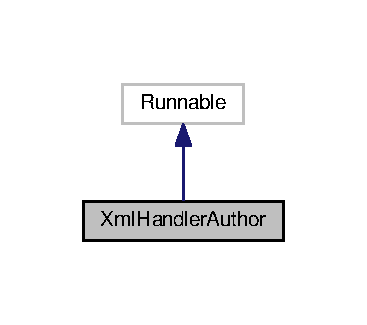
\includegraphics[width=176pt]{classXmlHandlerAuthor__inherit__graph}
\end{center}
\end{figure}


Collaboration diagram for Xml\-Handler\-Author\-:
\nopagebreak
\begin{figure}[H]
\begin{center}
\leavevmode
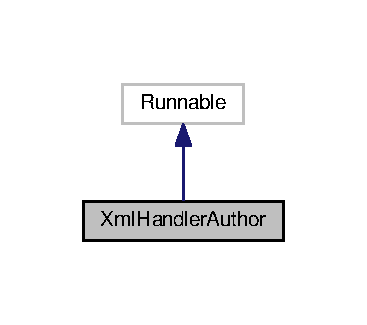
\includegraphics[width=176pt]{classXmlHandlerAuthor__coll__graph}
\end{center}
\end{figure}
\subsection*{Public Member Functions}
\begin{DoxyCompactItemize}
\item 
void \hyperlink{classXmlHandlerAuthor_a860da9fa6849b4dd8f362953faf14bcd}{find} (String str)
\item 
void \hyperlink{classXmlHandlerAuthor_ac509e27b7db234c3a8e6b537c05b0788}{set\-Category} (String cat)
\item 
void \hyperlink{classXmlHandlerAuthor_ae6dc18dbbb71e72db582f0964c655d74}{set\-Ee} (String e\-E)
\item 
void \hyperlink{classXmlHandlerAuthor_a34ffa560bb70eac46df935f5cdca6bcf}{set\-Pages} (String pag)
\item 
void \hyperlink{classXmlHandlerAuthor_a74cb8d94ee14ab382253abc5a38d6b8e}{set\-Year} (int y)
\item 
void \hyperlink{classXmlHandlerAuthor_a6137e5065cb6e2050ef6b9d1a2a50e48}{set\-Url} (String ur)
\item 
void \hyperlink{classXmlHandlerAuthor_afe6d790275f8d30f0ab3527b1aea934b}{set\-Title} (String t)
\item 
void \hyperlink{classXmlHandlerAuthor_a0635610c34233b096c4f47b5746a8d1c}{set\-Author} (String auth)
\item 
void \hyperlink{classXmlHandlerAuthor_a1e0a5b957fd643726ff122517e2d81c1}{set\-Volume} (String vol)
\item 
void \hyperlink{classXmlHandlerAuthor_acb7a439c54a29c688fc36190a529581f}{set\-Pub} (int x)
\item 
void \hyperlink{classXmlHandlerAuthor_ab9c56f83a382d3c70a0d3eb65e02272c}{search} (String str)
\item 
void \hyperlink{classXmlHandlerAuthor_adac17a195135fb961bb4a8b932138152}{start\-Element} (String uri, String local\-Name, String qname, Attributes attributes)  throws S\-A\-X\-Exception
\item 
void \hyperlink{classXmlHandlerAuthor_ad97c3844a098280d675ac0e703ac4e27}{characters} (char ch\-Array\mbox{[}$\,$\mbox{]}, int start, int length)
\item 
void \hyperlink{classXmlHandlerAuthor_ae6175824e08db40f2862bd06297d6847}{end\-Element} (String uri, String local\-Name, String qname)  throws S\-A\-X\-Exception
\item 
String \hyperlink{classXmlHandlerAuthor_a6f0222c5f34364a6c1d0906237cdf45a}{get\-Author} ()
\item 
String \hyperlink{classXmlHandlerAuthor_a6a6fd1aaef0587d30cff05dfa53da3c3}{get\-Title} ()
\item 
int \hyperlink{classXmlHandlerAuthor_a579ee55f6cf287873e1588943ab920f5}{get\-Year} ()
\item 
String \hyperlink{classXmlHandlerAuthor_acb036e9cc36cf8e042165ec28bfd6443}{get\-Pages} ()
\item 
String \hyperlink{classXmlHandlerAuthor_a6f3d4b439bce3ce234cfaa88a94d79ba}{get\-Volume} ()
\item 
String \hyperlink{classXmlHandlerAuthor_abbd48876dd5f44b21cbd716328b356a7}{get\-Journal} ()
\item 
String \hyperlink{classXmlHandlerAuthor_ae72e80845a09b05b609558a643c8d2d3}{get\-Url} ()
\item 
int \hyperlink{classXmlHandlerAuthor_aaef6b78de7e1405878268e8203807e5d}{get\-Number} ()
\item 
void \hyperlink{classXmlHandlerAuthor_a07d49493bfa706aabe10fe0f7927aa15}{find\-Auth} ()
\item 
Array\-List$<$ String $>$ \hyperlink{classXmlHandlerAuthor_a02f6252baeefc0e7b3458af0a1cde62a}{get\-Auth} ()
\item 
void \hyperlink{classXmlHandlerAuthor_a94447769489224e0cace8278d0fddeb2}{run} ()
\end{DoxyCompactItemize}
\subsection*{Public Attributes}
\begin{DoxyCompactItemize}
\item 
volatile int \hyperlink{classXmlHandlerAuthor_a3b5ed01d09eb68532c727613932065a8}{working}
\end{DoxyCompactItemize}


\subsection{Detailed Description}


Definition at line 9 of file Xml\-Handler.\-java.



\subsection{Member Function Documentation}
\hypertarget{classXmlHandlerAuthor_ad97c3844a098280d675ac0e703ac4e27}{\index{Xml\-Handler\-Author@{Xml\-Handler\-Author}!characters@{characters}}
\index{characters@{characters}!XmlHandlerAuthor@{Xml\-Handler\-Author}}
\subsubsection[{characters}]{\setlength{\rightskip}{0pt plus 5cm}void Xml\-Handler\-Author.\-characters (
\begin{DoxyParamCaption}
\item[{char}]{ch\-Array\mbox{[}$\,$\mbox{]}, }
\item[{int}]{start, }
\item[{int}]{length}
\end{DoxyParamCaption}
)\hspace{0.3cm}{\ttfamily [inline]}}}\label{classXmlHandlerAuthor_ad97c3844a098280d675ac0e703ac4e27}


Definition at line 223 of file Xml\-Handler.\-java.


\begin{DoxyCode}
223                                                                    \{
224         System.out.println(\textcolor{keyword}{new} String(chArray,start,length));
225             \textcolor{comment}{// if(flag == 0)\{}
226             \textcolor{comment}{//  author\_Name = new String (chArray,start,length);}
227             \textcolor{comment}{//  if(author\_Name.equals(author\_title))\{}
228             \textcolor{comment}{//      System.out.println("Author : " + author\_Name);}
229             \textcolor{comment}{//      flag = 1;}
230             \textcolor{comment}{//  \}}
231             \textcolor{comment}{// \}}
232             \textcolor{comment}{// else if(flag == 1 && !(title.isEmpty()))\{}
233             \textcolor{comment}{//  title\_String = new String(chArray,start,length);}
234             \textcolor{comment}{//  System.out.println("Title : " + title\_String);}
235             \textcolor{comment}{// \}}
236             \textcolor{comment}{// else if(flag == 1 && !(pages.isEmpty()))\{}
237             \textcolor{comment}{//  pages\_String = new String(chArray,start,length);}
238             \textcolor{comment}{//  System.out.println("Pages :" + pages\_String);}
239             \textcolor{comment}{// \}}
240             \textcolor{comment}{// else if(flag == 1 && !(year.isEmpty()))\{}
241             \textcolor{comment}{//  year\_String = new String(chArray,start,length);}
242             \textcolor{comment}{//  System.out.println("Year :" + year\_String);}
243             \textcolor{comment}{// \}}
244             \textcolor{comment}{// else if(flag == 1 && !(volume.isEmpty()))\{}
245             \textcolor{comment}{//  volume\_String = new String(chArray,start,length);}
246             \textcolor{comment}{//  System.out.println("Volume : " + volume\_String);}
247             \textcolor{comment}{// \}}
248             \textcolor{comment}{// else if(flag == 1 && !(journal.isEmpty()))\{}
249             \textcolor{comment}{//  journal\_String = new String(chArray,start,length);}
250             \textcolor{comment}{//  System.out.println("Journal : " + journal\_String);}
251             \textcolor{comment}{// \}}
252             \textcolor{comment}{// else if(flag == 1 && !(number.isEmpty()))\{}
253             \textcolor{comment}{//  number\_String = new String(chArray,start,length);}
254             \textcolor{comment}{//  System.out.println("Number :" + number\_String);}
255             \textcolor{comment}{// \}}
256             \textcolor{comment}{// else if(flag == 1 && !(url.isEmpty()))\{}
257             \textcolor{comment}{//  url\_String = new String(chArray,start,length);}
258             \textcolor{comment}{//  System.out.println("Url : " + url\_String);}
259             \textcolor{comment}{// \}}
260             \textcolor{comment}{// else if(flag == 1 && !(ee.isEmpty()))\{}
261             \textcolor{comment}{//  ee\_String = new String(chArray,start,length);}
262             \textcolor{comment}{//  System.out.println("ee : " + ee\_String);}
263             \textcolor{comment}{//  flag = 0;}
264             \textcolor{comment}{// \}}
265     \}
\end{DoxyCode}
\hypertarget{classXmlHandlerAuthor_ae6175824e08db40f2862bd06297d6847}{\index{Xml\-Handler\-Author@{Xml\-Handler\-Author}!end\-Element@{end\-Element}}
\index{end\-Element@{end\-Element}!XmlHandlerAuthor@{Xml\-Handler\-Author}}
\subsubsection[{end\-Element}]{\setlength{\rightskip}{0pt plus 5cm}void Xml\-Handler\-Author.\-end\-Element (
\begin{DoxyParamCaption}
\item[{String}]{uri, }
\item[{String}]{local\-Name, }
\item[{String}]{qname}
\end{DoxyParamCaption}
) throws S\-A\-X\-Exception\hspace{0.3cm}{\ttfamily [inline]}}}\label{classXmlHandlerAuthor_ae6175824e08db40f2862bd06297d6847}


Definition at line 266 of file Xml\-Handler.\-java.


\begin{DoxyCode}
266                                                                                          \{
267         \textcolor{keywordflow}{try}\{
268             \textcolor{comment}{// if(qname.equals("author"))\{}
269             \textcolor{comment}{//      author = new String();}
270             \textcolor{comment}{// \}}
271             \textcolor{comment}{// else if(qname.equals("title"))\{}
272             \textcolor{comment}{//  title = new String();}
273             \textcolor{comment}{// \}}
274             \textcolor{comment}{// else if(qname.equals("pages"))\{}
275             \textcolor{comment}{//  pages = new String();}
276             \textcolor{comment}{// \}}
277             \textcolor{comment}{// else if(qname.equals("year"))\{}
278             \textcolor{comment}{//  year = new String();}
279             \textcolor{comment}{// \}}
280             \textcolor{comment}{// else if(qname.equals("volume"))\{}
281             \textcolor{comment}{//  volume = new String();}
282             \textcolor{comment}{// \}}
283             \textcolor{comment}{// else if(qname.equals("journal"))\{}
284             \textcolor{comment}{//  journal = new String();}
285             \textcolor{comment}{// \}}
286             \textcolor{comment}{// else if(qname.equals("number"))\{}
287             \textcolor{comment}{//  number = new String();}
288             \textcolor{comment}{// \}}
289             \textcolor{comment}{// else if(qname.equals("url"))\{}
290             \textcolor{comment}{//  url = new String();}
291             \textcolor{comment}{// \}}
292             \textcolor{comment}{// else if(qname.equals("ee"))\{}
293             \textcolor{comment}{//  ee = new String();}
294             \textcolor{comment}{// \}}
295             System.out.println(qname);
296         \}
297         \textcolor{keywordflow}{catch}(Exception e)\{
298             e.printStackTrace();
299         \}
300     \}
\end{DoxyCode}
\hypertarget{classXmlHandlerAuthor_a860da9fa6849b4dd8f362953faf14bcd}{\index{Xml\-Handler\-Author@{Xml\-Handler\-Author}!find@{find}}
\index{find@{find}!XmlHandlerAuthor@{Xml\-Handler\-Author}}
\subsubsection[{find}]{\setlength{\rightskip}{0pt plus 5cm}void Xml\-Handler\-Author.\-find (
\begin{DoxyParamCaption}
\item[{String}]{str}
\end{DoxyParamCaption}
)\hspace{0.3cm}{\ttfamily [inline]}}}\label{classXmlHandlerAuthor_a860da9fa6849b4dd8f362953faf14bcd}


Definition at line 14 of file Xml\-Handler.\-java.


\begin{DoxyCode}
14                                 \{
15         \textcolor{keywordflow}{try}\{
16             SAXParserFactory fac = SAXParserFactory.newInstance();
17             SAXParser saxTheFile = factory.new SAXParser();
18             DefaultHandler defHandler = \textcolor{keyword}{new} DefaultHandler()\{
19                 
20                 \textcolor{comment}{// boolean checkAuth = false;}
21                 \textcolor{comment}{// boolean checkVal = false;}
22                 \textcolor{comment}{// boolean checkCat = false;}
23                 \textcolor{comment}{// boolean checkEe = false;}
24                 \textcolor{comment}{// boolean checkUrl = false;}
25                 \textcolor{comment}{// boolean checkPages = false;}
26                 \textcolor{comment}{// boolean checkVolume = false;}
27                 \textcolor{comment}{// boolean checkNumber = false;}
28                 \textcolor{comment}{// boolean checkYear = false;}
29                 \textcolor{comment}{// boolean checkTitle = false;}
30                 \textcolor{keywordtype}{boolean} checkCat = \textcolor{keyword}{false};
31                 \textcolor{keyword}{public} \textcolor{keywordtype}{void} \hyperlink{classXmlHandlerAuthor_adac17a195135fb961bb4a8b932138152}{startElement}(String uri,String localName,String qname,Attributes 
      att)\textcolor{keywordflow}{throws} SAXException\{
32                     \textcolor{keywordflow}{if}(qname.equals(\textcolor{stringliteral}{"www"}))\{
33                         \textcolor{comment}{// setCategory(qname);}
34                         checkCat = \textcolor{keyword}{true};
35                     \}
36                 \}
37                 \textcolor{keyword}{public} \textcolor{keywordtype}{void} \hyperlink{classXmlHandlerAuthor_ad97c3844a098280d675ac0e703ac4e27}{characters}(\textcolor{keywordtype}{char} chArray[],\textcolor{keywordtype}{int} start,\textcolor{keywordtype}{int} length)\textcolor{keywordflow}{throws} SAXException\{
38                     \textcolor{keywordflow}{if}(checkCat)\{
39                         
40                     \}
41                     \textcolor{keywordflow}{else} \textcolor{keywordflow}{if}(checkString)\{
42                         \textcolor{keywordflow}{if}(str.equals(\textcolor{keyword}{new} String(chArray,start,length)))\{
43                             checkVal = \textcolor{keyword}{true};
44                         \}
45                     \}
46                 \}
47                 \textcolor{keyword}{public} \textcolor{keywordtype}{void} \hyperlink{classXmlHandlerAuthor_ae6175824e08db40f2862bd06297d6847}{endElement}(String uri,String localName,String qname,Attributes att)\{
48                     
49                 \}
50             \}
51         \}
52         \textcolor{keywordflow}{catch}(Exception e)\{
53             e.printStackTrace();
54         \}
55     \}
\end{DoxyCode}
\hypertarget{classXmlHandlerAuthor_a07d49493bfa706aabe10fe0f7927aa15}{\index{Xml\-Handler\-Author@{Xml\-Handler\-Author}!find\-Auth@{find\-Auth}}
\index{find\-Auth@{find\-Auth}!XmlHandlerAuthor@{Xml\-Handler\-Author}}
\subsubsection[{find\-Auth}]{\setlength{\rightskip}{0pt plus 5cm}void Xml\-Handler\-Author.\-find\-Auth (
\begin{DoxyParamCaption}
{}
\end{DoxyParamCaption}
)\hspace{0.3cm}{\ttfamily [inline]}}}\label{classXmlHandlerAuthor_a07d49493bfa706aabe10fe0f7927aa15}


Definition at line 12 of file Xml\-Handler\-Author.\-java.


\begin{DoxyCode}
12                           \{
13         \textcolor{keywordflow}{try}\{
14             \hyperlink{classXmlHandlerAuthor_a3b5ed01d09eb68532c727613932065a8}{working} = 0;
15             System.setProperty(\textcolor{stringliteral}{"jdk.xml.entityExpansionLimit"}, \textcolor{stringliteral}{"0"});
16             SAXParserFactory fac = SAXParserFactory.newInstance();
17             SAXParser saxTheFile = fac.newSAXParser();
18             DefaultHandler defHandler = \textcolor{keyword}{new} DefaultHandler()\{
19                 ArrayList<String> temp = \textcolor{keyword}{new} ArrayList<>();
20                 \textcolor{keywordtype}{int} counter = 0;
21                 String snum;
22                 \textcolor{keywordtype}{boolean} checkCat = \textcolor{keyword}{false},checkAuth = \textcolor{keyword}{false},checkString = \textcolor{keyword}{true},checkTitle = \textcolor{keyword}{false},check = \textcolor{keyword}{
      false};
23                 \textcolor{keyword}{public} \textcolor{keywordtype}{void} \hyperlink{classXmlHandlerAuthor_adac17a195135fb961bb4a8b932138152}{startElement}(String uri,String localName,String qname,Attributes 
      att)\textcolor{keywordflow}{throws} SAXException\{
24                     \textcolor{keywordflow}{if}(qname.equals(\textcolor{stringliteral}{"www"}))\{
25                         checkCat = \textcolor{keyword}{true};
26                         checkTitle = \textcolor{keyword}{false};
27                     \}
28                     \textcolor{keywordflow}{else} \textcolor{keywordflow}{if}(qname.equals(\textcolor{stringliteral}{"author"}) && checkCat)\{
29                         checkAuth = \textcolor{keyword}{true};
30                         join=\textcolor{stringliteral}{""};
31                     \}
32                     \textcolor{keywordflow}{else} \textcolor{keywordflow}{if}(qname.equals(\textcolor{stringliteral}{"title"}) && checkCat)\{
33                         checkTitle = \textcolor{keyword}{true};
34                     \}
35                 \}
36                 \textcolor{keyword}{public} \textcolor{keywordtype}{void} \hyperlink{classXmlHandlerAuthor_ad97c3844a098280d675ac0e703ac4e27}{characters}(\textcolor{keywordtype}{char} chArray[],\textcolor{keywordtype}{int} start,\textcolor{keywordtype}{int} length)\textcolor{keywordflow}{throws} SAXException\{
37                     \textcolor{keywordflow}{if}(checkCat && checkAuth)\{
38                         String auth = \textcolor{keyword}{new} String(chArray,start,length);
39                         join = join+auth;
40                         
41                     \}
42                     \textcolor{keywordflow}{else} \textcolor{keywordflow}{if}(checkTitle)\{
43                         \textcolor{keywordflow}{if}((\textcolor{keyword}{new} String(chArray,start,length)).equals(\textcolor{stringliteral}{"Home Page"}))\{
44                             check = \textcolor{keyword}{true};
45                         \}
46                     \}
47                 \}
48                 \textcolor{keyword}{public} \textcolor{keywordtype}{void} \hyperlink{classXmlHandlerAuthor_ae6175824e08db40f2862bd06297d6847}{endElement}(String uri,String localName,String qname)\textcolor{keywordflow}{throws} 
      SAXException\{
49                     \textcolor{keywordflow}{if}(qname.equals(\textcolor{stringliteral}{"author"}))\{
50                         checkAuth = \textcolor{keyword}{false};
51                         temp.add(join);
52                     \}
53                     \textcolor{keywordflow}{else} \textcolor{keywordflow}{if}(qname.equals(\textcolor{stringliteral}{"www"}))\{
54                         \textcolor{keywordflow}{if}(checkString && check)\{
55                             author.addAll(temp);
56                             counter = counter + 1;
57                             snum = Integer.toString(counter);
58                             writer(snum,author);
59                             check = \textcolor{keyword}{false};
60                             author.clear();
61                             temp.clear();
62                         \}
63                         \textcolor{keywordflow}{else} \textcolor{keywordflow}{if}(checkString == \textcolor{keyword}{false} || check == \textcolor{keyword}{false})\{
64                             temp.clear();
65                             check = \textcolor{keyword}{false};
66                         \}
67                         check = \textcolor{keyword}{false};
68                         checkCat = \textcolor{keyword}{false};
69                     \}
70                 \}
71             \};
72             saxTheFile.parse(\textcolor{stringliteral}{"dblp.xml"},defHandler);
73         \}
74         \textcolor{keywordflow}{catch}(Exception e)\{
75             e.printStackTrace();
76         \}
77         \textcolor{keywordflow}{finally}\{
78             \hyperlink{classXmlHandlerAuthor_a3b5ed01d09eb68532c727613932065a8}{working} = 1;
79         \}
80     \}
\end{DoxyCode}
\hypertarget{classXmlHandlerAuthor_a02f6252baeefc0e7b3458af0a1cde62a}{\index{Xml\-Handler\-Author@{Xml\-Handler\-Author}!get\-Auth@{get\-Auth}}
\index{get\-Auth@{get\-Auth}!XmlHandlerAuthor@{Xml\-Handler\-Author}}
\subsubsection[{get\-Auth}]{\setlength{\rightskip}{0pt plus 5cm}Array\-List$<$String$>$ Xml\-Handler\-Author.\-get\-Auth (
\begin{DoxyParamCaption}
{}
\end{DoxyParamCaption}
)\hspace{0.3cm}{\ttfamily [inline]}}}\label{classXmlHandlerAuthor_a02f6252baeefc0e7b3458af0a1cde62a}


Definition at line 97 of file Xml\-Handler\-Author.\-java.


\begin{DoxyCode}
97                                       \{
98         \textcolor{keywordflow}{return} author;
99     \}
\end{DoxyCode}
\hypertarget{classXmlHandlerAuthor_a6f0222c5f34364a6c1d0906237cdf45a}{\index{Xml\-Handler\-Author@{Xml\-Handler\-Author}!get\-Author@{get\-Author}}
\index{get\-Author@{get\-Author}!XmlHandlerAuthor@{Xml\-Handler\-Author}}
\subsubsection[{get\-Author}]{\setlength{\rightskip}{0pt plus 5cm}String Xml\-Handler\-Author.\-get\-Author (
\begin{DoxyParamCaption}
{}
\end{DoxyParamCaption}
)\hspace{0.3cm}{\ttfamily [inline]}}}\label{classXmlHandlerAuthor_a6f0222c5f34364a6c1d0906237cdf45a}


Definition at line 301 of file Xml\-Handler.\-java.


\begin{DoxyCode}
301                              \{
302         \textcolor{keywordflow}{return} author\_Name;
303     \}
\end{DoxyCode}
\hypertarget{classXmlHandlerAuthor_abbd48876dd5f44b21cbd716328b356a7}{\index{Xml\-Handler\-Author@{Xml\-Handler\-Author}!get\-Journal@{get\-Journal}}
\index{get\-Journal@{get\-Journal}!XmlHandlerAuthor@{Xml\-Handler\-Author}}
\subsubsection[{get\-Journal}]{\setlength{\rightskip}{0pt plus 5cm}String Xml\-Handler\-Author.\-get\-Journal (
\begin{DoxyParamCaption}
{}
\end{DoxyParamCaption}
)\hspace{0.3cm}{\ttfamily [inline]}}}\label{classXmlHandlerAuthor_abbd48876dd5f44b21cbd716328b356a7}


Definition at line 317 of file Xml\-Handler.\-java.


\begin{DoxyCode}
317                               \{
318         \textcolor{keywordflow}{return} journal\_String;
319     \}
\end{DoxyCode}
\hypertarget{classXmlHandlerAuthor_aaef6b78de7e1405878268e8203807e5d}{\index{Xml\-Handler\-Author@{Xml\-Handler\-Author}!get\-Number@{get\-Number}}
\index{get\-Number@{get\-Number}!XmlHandlerAuthor@{Xml\-Handler\-Author}}
\subsubsection[{get\-Number}]{\setlength{\rightskip}{0pt plus 5cm}int Xml\-Handler\-Author.\-get\-Number (
\begin{DoxyParamCaption}
{}
\end{DoxyParamCaption}
)\hspace{0.3cm}{\ttfamily [inline]}}}\label{classXmlHandlerAuthor_aaef6b78de7e1405878268e8203807e5d}


Definition at line 323 of file Xml\-Handler.\-java.


\begin{DoxyCode}
323                           \{
324         \textcolor{keywordtype}{int} x = Integer.parseInt(number\_String);
325         \textcolor{keywordflow}{return} x;
326     \}
\end{DoxyCode}
\hypertarget{classXmlHandlerAuthor_acb036e9cc36cf8e042165ec28bfd6443}{\index{Xml\-Handler\-Author@{Xml\-Handler\-Author}!get\-Pages@{get\-Pages}}
\index{get\-Pages@{get\-Pages}!XmlHandlerAuthor@{Xml\-Handler\-Author}}
\subsubsection[{get\-Pages}]{\setlength{\rightskip}{0pt plus 5cm}String Xml\-Handler\-Author.\-get\-Pages (
\begin{DoxyParamCaption}
{}
\end{DoxyParamCaption}
)\hspace{0.3cm}{\ttfamily [inline]}}}\label{classXmlHandlerAuthor_acb036e9cc36cf8e042165ec28bfd6443}


Definition at line 311 of file Xml\-Handler.\-java.


\begin{DoxyCode}
311                             \{
312         \textcolor{keywordflow}{return} pages\_String;
313     \}
\end{DoxyCode}
\hypertarget{classXmlHandlerAuthor_a6a6fd1aaef0587d30cff05dfa53da3c3}{\index{Xml\-Handler\-Author@{Xml\-Handler\-Author}!get\-Title@{get\-Title}}
\index{get\-Title@{get\-Title}!XmlHandlerAuthor@{Xml\-Handler\-Author}}
\subsubsection[{get\-Title}]{\setlength{\rightskip}{0pt plus 5cm}String Xml\-Handler\-Author.\-get\-Title (
\begin{DoxyParamCaption}
{}
\end{DoxyParamCaption}
)\hspace{0.3cm}{\ttfamily [inline]}}}\label{classXmlHandlerAuthor_a6a6fd1aaef0587d30cff05dfa53da3c3}


Definition at line 304 of file Xml\-Handler.\-java.


\begin{DoxyCode}
304                             \{
305         \textcolor{keywordflow}{return} title\_String;
306     \}
\end{DoxyCode}
\hypertarget{classXmlHandlerAuthor_ae72e80845a09b05b609558a643c8d2d3}{\index{Xml\-Handler\-Author@{Xml\-Handler\-Author}!get\-Url@{get\-Url}}
\index{get\-Url@{get\-Url}!XmlHandlerAuthor@{Xml\-Handler\-Author}}
\subsubsection[{get\-Url}]{\setlength{\rightskip}{0pt plus 5cm}String Xml\-Handler\-Author.\-get\-Url (
\begin{DoxyParamCaption}
{}
\end{DoxyParamCaption}
)\hspace{0.3cm}{\ttfamily [inline]}}}\label{classXmlHandlerAuthor_ae72e80845a09b05b609558a643c8d2d3}


Definition at line 320 of file Xml\-Handler.\-java.


\begin{DoxyCode}
320                           \{
321         \textcolor{keywordflow}{return} url\_String;
322     \}
\end{DoxyCode}
\hypertarget{classXmlHandlerAuthor_a6f3d4b439bce3ce234cfaa88a94d79ba}{\index{Xml\-Handler\-Author@{Xml\-Handler\-Author}!get\-Volume@{get\-Volume}}
\index{get\-Volume@{get\-Volume}!XmlHandlerAuthor@{Xml\-Handler\-Author}}
\subsubsection[{get\-Volume}]{\setlength{\rightskip}{0pt plus 5cm}String Xml\-Handler\-Author.\-get\-Volume (
\begin{DoxyParamCaption}
{}
\end{DoxyParamCaption}
)\hspace{0.3cm}{\ttfamily [inline]}}}\label{classXmlHandlerAuthor_a6f3d4b439bce3ce234cfaa88a94d79ba}


Definition at line 314 of file Xml\-Handler.\-java.


\begin{DoxyCode}
314                              \{
315         \textcolor{keywordflow}{return} volume\_String;
316     \}
\end{DoxyCode}
\hypertarget{classXmlHandlerAuthor_a579ee55f6cf287873e1588943ab920f5}{\index{Xml\-Handler\-Author@{Xml\-Handler\-Author}!get\-Year@{get\-Year}}
\index{get\-Year@{get\-Year}!XmlHandlerAuthor@{Xml\-Handler\-Author}}
\subsubsection[{get\-Year}]{\setlength{\rightskip}{0pt plus 5cm}int Xml\-Handler\-Author.\-get\-Year (
\begin{DoxyParamCaption}
{}
\end{DoxyParamCaption}
)\hspace{0.3cm}{\ttfamily [inline]}}}\label{classXmlHandlerAuthor_a579ee55f6cf287873e1588943ab920f5}


Definition at line 307 of file Xml\-Handler.\-java.


\begin{DoxyCode}
307                         \{
308         \textcolor{keywordtype}{int} y = Integer.parseInt(year\_String);
309         \textcolor{keywordflow}{return} y;
310     \}
\end{DoxyCode}
\hypertarget{classXmlHandlerAuthor_a94447769489224e0cace8278d0fddeb2}{\index{Xml\-Handler\-Author@{Xml\-Handler\-Author}!run@{run}}
\index{run@{run}!XmlHandlerAuthor@{Xml\-Handler\-Author}}
\subsubsection[{run}]{\setlength{\rightskip}{0pt plus 5cm}void Xml\-Handler\-Author.\-run (
\begin{DoxyParamCaption}
{}
\end{DoxyParamCaption}
)\hspace{0.3cm}{\ttfamily [inline]}}}\label{classXmlHandlerAuthor_a94447769489224e0cace8278d0fddeb2}


Definition at line 101 of file Xml\-Handler\-Author.\-java.


\begin{DoxyCode}
101                       \{
102     \hyperlink{classXmlHandlerAuthor_a07d49493bfa706aabe10fe0f7927aa15}{findAuth}();     
103     \}
\end{DoxyCode}
\hypertarget{classXmlHandlerAuthor_ab9c56f83a382d3c70a0d3eb65e02272c}{\index{Xml\-Handler\-Author@{Xml\-Handler\-Author}!search@{search}}
\index{search@{search}!XmlHandlerAuthor@{Xml\-Handler\-Author}}
\subsubsection[{search}]{\setlength{\rightskip}{0pt plus 5cm}void Xml\-Handler\-Author.\-search (
\begin{DoxyParamCaption}
\item[{String}]{str}
\end{DoxyParamCaption}
)\hspace{0.3cm}{\ttfamily [inline]}}}\label{classXmlHandlerAuthor_ab9c56f83a382d3c70a0d3eb65e02272c}


Definition at line 182 of file Xml\-Handler.\-java.


\begin{DoxyCode}
182                                   \{
183         author\_title = str;
184         strLength = author\_title.length();
185     \}
\end{DoxyCode}
\hypertarget{classXmlHandlerAuthor_a0635610c34233b096c4f47b5746a8d1c}{\index{Xml\-Handler\-Author@{Xml\-Handler\-Author}!set\-Author@{set\-Author}}
\index{set\-Author@{set\-Author}!XmlHandlerAuthor@{Xml\-Handler\-Author}}
\subsubsection[{set\-Author}]{\setlength{\rightskip}{0pt plus 5cm}void Xml\-Handler\-Author.\-set\-Author (
\begin{DoxyParamCaption}
\item[{String}]{auth}
\end{DoxyParamCaption}
)\hspace{0.3cm}{\ttfamily [inline]}}}\label{classXmlHandlerAuthor_a0635610c34233b096c4f47b5746a8d1c}


Definition at line 74 of file Xml\-Handler.\-java.


\begin{DoxyCode}
74                                       \{
75         author = auth;
76     \}
\end{DoxyCode}
\hypertarget{classXmlHandlerAuthor_ac509e27b7db234c3a8e6b537c05b0788}{\index{Xml\-Handler\-Author@{Xml\-Handler\-Author}!set\-Category@{set\-Category}}
\index{set\-Category@{set\-Category}!XmlHandlerAuthor@{Xml\-Handler\-Author}}
\subsubsection[{set\-Category}]{\setlength{\rightskip}{0pt plus 5cm}void Xml\-Handler\-Author.\-set\-Category (
\begin{DoxyParamCaption}
\item[{String}]{cat}
\end{DoxyParamCaption}
)\hspace{0.3cm}{\ttfamily [inline]}}}\label{classXmlHandlerAuthor_ac509e27b7db234c3a8e6b537c05b0788}


Definition at line 56 of file Xml\-Handler.\-java.


\begin{DoxyCode}
56                                        \{
57         category = cat;
58     \}
\end{DoxyCode}
\hypertarget{classXmlHandlerAuthor_ae6dc18dbbb71e72db582f0964c655d74}{\index{Xml\-Handler\-Author@{Xml\-Handler\-Author}!set\-Ee@{set\-Ee}}
\index{set\-Ee@{set\-Ee}!XmlHandlerAuthor@{Xml\-Handler\-Author}}
\subsubsection[{set\-Ee}]{\setlength{\rightskip}{0pt plus 5cm}void Xml\-Handler\-Author.\-set\-Ee (
\begin{DoxyParamCaption}
\item[{String}]{e\-E}
\end{DoxyParamCaption}
)\hspace{0.3cm}{\ttfamily [inline]}}}\label{classXmlHandlerAuthor_ae6dc18dbbb71e72db582f0964c655d74}


Definition at line 59 of file Xml\-Handler.\-java.


\begin{DoxyCode}
59                                 \{
60         ee = eE;
61     \}
\end{DoxyCode}
\hypertarget{classXmlHandlerAuthor_a34ffa560bb70eac46df935f5cdca6bcf}{\index{Xml\-Handler\-Author@{Xml\-Handler\-Author}!set\-Pages@{set\-Pages}}
\index{set\-Pages@{set\-Pages}!XmlHandlerAuthor@{Xml\-Handler\-Author}}
\subsubsection[{set\-Pages}]{\setlength{\rightskip}{0pt plus 5cm}void Xml\-Handler\-Author.\-set\-Pages (
\begin{DoxyParamCaption}
\item[{String}]{pag}
\end{DoxyParamCaption}
)\hspace{0.3cm}{\ttfamily [inline]}}}\label{classXmlHandlerAuthor_a34ffa560bb70eac46df935f5cdca6bcf}


Definition at line 62 of file Xml\-Handler.\-java.


\begin{DoxyCode}
62                                     \{
63         pages = pag;
64     \}
\end{DoxyCode}
\hypertarget{classXmlHandlerAuthor_acb7a439c54a29c688fc36190a529581f}{\index{Xml\-Handler\-Author@{Xml\-Handler\-Author}!set\-Pub@{set\-Pub}}
\index{set\-Pub@{set\-Pub}!XmlHandlerAuthor@{Xml\-Handler\-Author}}
\subsubsection[{set\-Pub}]{\setlength{\rightskip}{0pt plus 5cm}void Xml\-Handler\-Author.\-set\-Pub (
\begin{DoxyParamCaption}
\item[{int}]{x}
\end{DoxyParamCaption}
)\hspace{0.3cm}{\ttfamily [inline]}}}\label{classXmlHandlerAuthor_acb7a439c54a29c688fc36190a529581f}


Definition at line 80 of file Xml\-Handler.\-java.


\begin{DoxyCode}
80                              \{
81         publication = x;
82     \}
\end{DoxyCode}
\hypertarget{classXmlHandlerAuthor_afe6d790275f8d30f0ab3527b1aea934b}{\index{Xml\-Handler\-Author@{Xml\-Handler\-Author}!set\-Title@{set\-Title}}
\index{set\-Title@{set\-Title}!XmlHandlerAuthor@{Xml\-Handler\-Author}}
\subsubsection[{set\-Title}]{\setlength{\rightskip}{0pt plus 5cm}void Xml\-Handler\-Author.\-set\-Title (
\begin{DoxyParamCaption}
\item[{String}]{t}
\end{DoxyParamCaption}
)\hspace{0.3cm}{\ttfamily [inline]}}}\label{classXmlHandlerAuthor_afe6d790275f8d30f0ab3527b1aea934b}


Definition at line 71 of file Xml\-Handler.\-java.


\begin{DoxyCode}
71                                   \{
72         title = t;
73     \}
\end{DoxyCode}
\hypertarget{classXmlHandlerAuthor_a6137e5065cb6e2050ef6b9d1a2a50e48}{\index{Xml\-Handler\-Author@{Xml\-Handler\-Author}!set\-Url@{set\-Url}}
\index{set\-Url@{set\-Url}!XmlHandlerAuthor@{Xml\-Handler\-Author}}
\subsubsection[{set\-Url}]{\setlength{\rightskip}{0pt plus 5cm}void Xml\-Handler\-Author.\-set\-Url (
\begin{DoxyParamCaption}
\item[{String}]{ur}
\end{DoxyParamCaption}
)\hspace{0.3cm}{\ttfamily [inline]}}}\label{classXmlHandlerAuthor_a6137e5065cb6e2050ef6b9d1a2a50e48}


Definition at line 68 of file Xml\-Handler.\-java.


\begin{DoxyCode}
68                                  \{
69         url = ur;
70     \}
\end{DoxyCode}
\hypertarget{classXmlHandlerAuthor_a1e0a5b957fd643726ff122517e2d81c1}{\index{Xml\-Handler\-Author@{Xml\-Handler\-Author}!set\-Volume@{set\-Volume}}
\index{set\-Volume@{set\-Volume}!XmlHandlerAuthor@{Xml\-Handler\-Author}}
\subsubsection[{set\-Volume}]{\setlength{\rightskip}{0pt plus 5cm}void Xml\-Handler\-Author.\-set\-Volume (
\begin{DoxyParamCaption}
\item[{String}]{vol}
\end{DoxyParamCaption}
)\hspace{0.3cm}{\ttfamily [inline]}}}\label{classXmlHandlerAuthor_a1e0a5b957fd643726ff122517e2d81c1}


Definition at line 77 of file Xml\-Handler.\-java.


\begin{DoxyCode}
77                                      \{
78         volume = vol;
79     \}
\end{DoxyCode}
\hypertarget{classXmlHandlerAuthor_a74cb8d94ee14ab382253abc5a38d6b8e}{\index{Xml\-Handler\-Author@{Xml\-Handler\-Author}!set\-Year@{set\-Year}}
\index{set\-Year@{set\-Year}!XmlHandlerAuthor@{Xml\-Handler\-Author}}
\subsubsection[{set\-Year}]{\setlength{\rightskip}{0pt plus 5cm}void Xml\-Handler\-Author.\-set\-Year (
\begin{DoxyParamCaption}
\item[{int}]{y}
\end{DoxyParamCaption}
)\hspace{0.3cm}{\ttfamily [inline]}}}\label{classXmlHandlerAuthor_a74cb8d94ee14ab382253abc5a38d6b8e}


Definition at line 65 of file Xml\-Handler.\-java.


\begin{DoxyCode}
65                               \{
66         year = y;
67     \}
\end{DoxyCode}
\hypertarget{classXmlHandlerAuthor_adac17a195135fb961bb4a8b932138152}{\index{Xml\-Handler\-Author@{Xml\-Handler\-Author}!start\-Element@{start\-Element}}
\index{start\-Element@{start\-Element}!XmlHandlerAuthor@{Xml\-Handler\-Author}}
\subsubsection[{start\-Element}]{\setlength{\rightskip}{0pt plus 5cm}void Xml\-Handler\-Author.\-start\-Element (
\begin{DoxyParamCaption}
\item[{String}]{uri, }
\item[{String}]{local\-Name, }
\item[{String}]{qname, }
\item[{Attributes}]{attributes}
\end{DoxyParamCaption}
) throws S\-A\-X\-Exception\hspace{0.3cm}{\ttfamily [inline]}}}\label{classXmlHandlerAuthor_adac17a195135fb961bb4a8b932138152}


Definition at line 186 of file Xml\-Handler.\-java.


\begin{DoxyCode}
186                                                                                                            
               \{
187         \textcolor{keywordflow}{try}\{
188             System.out.println(qname);
189             \textcolor{comment}{// if(!author\_title.isEmpty())\{}
190             \textcolor{comment}{//  if(qname.equals("author"))\{}
191             \textcolor{comment}{//      author = qname;}
192             \textcolor{comment}{//  \}}
193             \textcolor{comment}{//  else if(qname.equals("title"))\{}
194             \textcolor{comment}{//      title = qname;}
195             \textcolor{comment}{//  \}}
196             \textcolor{comment}{//  else if(qname.equals("pages"))\{}
197             \textcolor{comment}{//      pages = qname;}
198             \textcolor{comment}{//  \}}
199             \textcolor{comment}{//  else if(qname.equals("year"))\{}
200             \textcolor{comment}{//      year = qname;}
201             \textcolor{comment}{//  \}}
202             \textcolor{comment}{//  else if(qname.equals("volume"))\{}
203             \textcolor{comment}{//      volume = qname;}
204             \textcolor{comment}{//  \}}
205             \textcolor{comment}{//  else if(qname.equals("journal"))\{}
206             \textcolor{comment}{//      journal = qname;}
207             \textcolor{comment}{//  \}}
208             \textcolor{comment}{//  else if(qname.equals("number"))\{}
209             \textcolor{comment}{//      number = qname;}
210             \textcolor{comment}{//  \}}
211             \textcolor{comment}{//  else if(qname.equals("url"))\{}
212             \textcolor{comment}{//      url = qname;}
213             \textcolor{comment}{//  \}}
214             \textcolor{comment}{//  else if(qname.equals("ee"))\{}
215             \textcolor{comment}{//      ee = qname;}
216             \textcolor{comment}{//  \}}
217             \textcolor{comment}{// \}}
218         \}
219         \textcolor{keywordflow}{catch}(Exception e)\{
220             e.printStackTrace();
221         \}
222     \}
\end{DoxyCode}


\subsection{Member Data Documentation}
\hypertarget{classXmlHandlerAuthor_a3b5ed01d09eb68532c727613932065a8}{\index{Xml\-Handler\-Author@{Xml\-Handler\-Author}!working@{working}}
\index{working@{working}!XmlHandlerAuthor@{Xml\-Handler\-Author}}
\subsubsection[{working}]{\setlength{\rightskip}{0pt plus 5cm}volatile int Xml\-Handler\-Author.\-working}}\label{classXmlHandlerAuthor_a3b5ed01d09eb68532c727613932065a8}


Definition at line 11 of file Xml\-Handler\-Author.\-java.



The documentation for this class was generated from the following files\-:\begin{DoxyCompactItemize}
\item 
\hyperlink{XmlHandler_8java}{Xml\-Handler.\-java}\item 
\hyperlink{XmlHandlerAuthor_8java}{Xml\-Handler\-Author.\-java}\end{DoxyCompactItemize}

\hypertarget{classXmlHandlerTitle}{\section{Xml\-Handler\-Title Class Reference}
\label{classXmlHandlerTitle}\index{Xml\-Handler\-Title@{Xml\-Handler\-Title}}
}


Inheritance diagram for Xml\-Handler\-Title\-:
\nopagebreak
\begin{figure}[H]
\begin{center}
\leavevmode
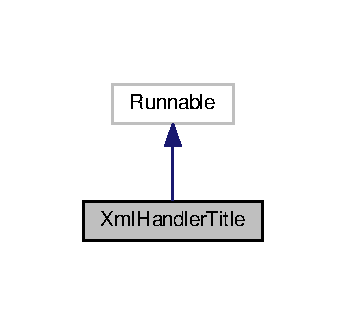
\includegraphics[width=166pt]{classXmlHandlerTitle__inherit__graph}
\end{center}
\end{figure}


Collaboration diagram for Xml\-Handler\-Title\-:
\nopagebreak
\begin{figure}[H]
\begin{center}
\leavevmode
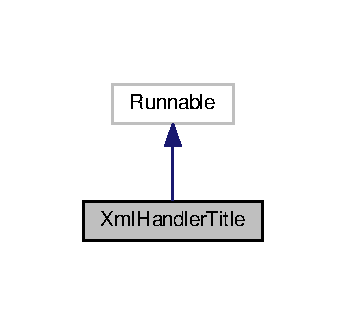
\includegraphics[width=166pt]{classXmlHandlerTitle__coll__graph}
\end{center}
\end{figure}
\subsection*{Public Member Functions}
\begin{DoxyCompactItemize}
\item 
\hyperlink{classXmlHandlerTitle_a41d8f5e4c21f2e3d9846593d1d7d5da6}{Xml\-Handler\-Title} (String x, int y)
\item 
void \hyperlink{classXmlHandlerTitle_a8bb351908c7504b82dc0dbfcfff5352c}{find\-Title} ()
\item 
void \hyperlink{classXmlHandlerTitle_a5ae3c12233674e2953bbfc51d19084c7}{sort} ()
\item 
void \hyperlink{classXmlHandlerTitle_ac7189c60a6cad49f37cac7a1b994abda}{run} ()
\end{DoxyCompactItemize}
\subsection*{Public Attributes}
\begin{DoxyCompactItemize}
\item 
volatile int \hyperlink{classXmlHandlerTitle_a8430143db4f1036e5db03fbe7e3d451f}{working}
\end{DoxyCompactItemize}


\subsection{Detailed Description}


Definition at line 8 of file Xml\-Handler\-Title.\-java.



\subsection{Constructor \& Destructor Documentation}
\hypertarget{classXmlHandlerTitle_a41d8f5e4c21f2e3d9846593d1d7d5da6}{\index{Xml\-Handler\-Title@{Xml\-Handler\-Title}!Xml\-Handler\-Title@{Xml\-Handler\-Title}}
\index{Xml\-Handler\-Title@{Xml\-Handler\-Title}!XmlHandlerTitle@{Xml\-Handler\-Title}}
\subsubsection[{Xml\-Handler\-Title}]{\setlength{\rightskip}{0pt plus 5cm}Xml\-Handler\-Title.\-Xml\-Handler\-Title (
\begin{DoxyParamCaption}
\item[{String}]{x, }
\item[{int}]{y}
\end{DoxyParamCaption}
)\hspace{0.3cm}{\ttfamily [inline]}}}\label{classXmlHandlerTitle_a41d8f5e4c21f2e3d9846593d1d7d5da6}


Definition at line 14 of file Xml\-Handler\-Title.\-java.


\begin{DoxyCode}
14                                           \{
15         this.str = x;
16         this.type = y;
17     \}
\end{DoxyCode}


\subsection{Member Function Documentation}
\hypertarget{classXmlHandlerTitle_a8bb351908c7504b82dc0dbfcfff5352c}{\index{Xml\-Handler\-Title@{Xml\-Handler\-Title}!find\-Title@{find\-Title}}
\index{find\-Title@{find\-Title}!XmlHandlerTitle@{Xml\-Handler\-Title}}
\subsubsection[{find\-Title}]{\setlength{\rightskip}{0pt plus 5cm}void Xml\-Handler\-Title.\-find\-Title (
\begin{DoxyParamCaption}
{}
\end{DoxyParamCaption}
)\hspace{0.3cm}{\ttfamily [inline]}}}\label{classXmlHandlerTitle_a8bb351908c7504b82dc0dbfcfff5352c}


Definition at line 18 of file Xml\-Handler\-Title.\-java.


\begin{DoxyCode}
18                            \{
19         \textcolor{keywordflow}{try}\{
20             \hyperlink{classXmlHandlerTitle_a8430143db4f1036e5db03fbe7e3d451f}{working} = 0;
21             System.setProperty(\textcolor{stringliteral}{"jdk.xml.entityExpansionLimit"}, \textcolor{stringliteral}{"0"});
22             PrintWriter write = \textcolor{keyword}{new} PrintWriter( \textcolor{keyword}{new} BufferedWriter( \textcolor{keyword}{new} FileWriter ( \textcolor{stringliteral}{"Ref.txt"}) ) );
23             write.close();
24             SAXParserFactory fac = SAXParserFactory.newInstance();
25             SAXParser saxTheFile = fac.newSAXParser();
26             DefaultHandler defHandler = \textcolor{keyword}{new} DefaultHandler()\{
27                 String title,pages,url,volume,year,snum,journal;
28                 \textcolor{keywordtype}{int} counter=0;
29                 \textcolor{keywordtype}{boolean} titleCheck = \textcolor{keyword}{false},relcheck=\textcolor{keyword}{false},volCheck = \textcolor{keyword}{false},yearCheck = \textcolor{keyword}{false},urlCheck = \textcolor{keyword}{
      false},checkAuth = \textcolor{keyword}{false},pagesCheck = \textcolor{keyword}{false}, journalCheck = \textcolor{keyword}{false},checkCat = \textcolor{keyword}{true};
30                 \textcolor{keyword}{public} \textcolor{keywordtype}{void} startElement(String uri,String localName,String qname,Attributes att)\textcolor{keywordflow}{throws} 
      SAXException\{
31                     \textcolor{keywordflow}{if}(qname.equals(\textcolor{stringliteral}{"www"}))\{
32                         checkCat = \textcolor{keyword}{false};
33                     \}
34                     \textcolor{keywordflow}{else} \textcolor{keywordflow}{if}(qname.equals(\textcolor{stringliteral}{"author"}) || qname.equals(\textcolor{stringliteral}{"editor"}))\{
35                         checkAuth = \textcolor{keyword}{true};
36                         join = \textcolor{stringliteral}{""};
37                     \}
38                     \textcolor{keywordflow}{else} \textcolor{keywordflow}{if}(qname.equals(\textcolor{stringliteral}{"title"}))\{
39                         titleCheck = \textcolor{keyword}{true};
40                     \}
41                     \textcolor{keywordflow}{else} \textcolor{keywordflow}{if}(qname.equals(\textcolor{stringliteral}{"year"}))\{
42                         yearCheck = \textcolor{keyword}{true};
43                     \}
44                     \textcolor{keywordflow}{else} \textcolor{keywordflow}{if}(qname.equals(\textcolor{stringliteral}{"url"}))\{
45                         urlCheck = \textcolor{keyword}{true};
46                     \}
47                     \textcolor{keywordflow}{else} \textcolor{keywordflow}{if}(qname.equals(\textcolor{stringliteral}{"pages"}))\{
48                         pagesCheck = \textcolor{keyword}{true};
49                     \}
50                     \textcolor{keywordflow}{else} \textcolor{keywordflow}{if}(qname.equals(\textcolor{stringliteral}{"volume"}))\{
51                         volCheck = \textcolor{keyword}{true};
52                     \}
53                     \textcolor{keywordflow}{else} \textcolor{keywordflow}{if}(qname.equals(\textcolor{stringliteral}{"journal"}) || qname.equals(\textcolor{stringliteral}{"booktitle"}))\{
54                         journalCheck = \textcolor{keyword}{true};
55                     \}
56                 \}
57                 \textcolor{keyword}{public} \textcolor{keywordtype}{void} characters(\textcolor{keywordtype}{char} chArray[],\textcolor{keywordtype}{int} start,\textcolor{keywordtype}{int} length)\textcolor{keywordflow}{throws} SAXException\{
58                     \textcolor{keywordflow}{if}(checkAuth && checkCat)\{
59                         String temp = \textcolor{keyword}{new} String(chArray,start,length); 
60                         join = join+temp;
61                     \}
62                     \textcolor{keywordflow}{else} \textcolor{keywordflow}{if}(titleCheck && checkCat)\{
63                         title = \textcolor{keyword}{new} String(chArray,start,length);
64                         String tempArray[] = str.split(\textcolor{stringliteral}{" "});
65                         \textcolor{keywordtype}{int} i= 0;
66                         \textcolor{keywordflow}{for}(i=0;i<tempArray.length;i++)\{
67                             \textcolor{keywordflow}{if}(tempArray[i].length() >= 4)\{
68                                 String titleArray [] = title.split(\textcolor{stringliteral}{" "});
69                                 \textcolor{keywordtype}{int} j;
70                                 \textcolor{keywordflow}{for}(j=0;j<titleArray.length;j++)\{
71                                     titleArray[j] = titleArray[j].replace(\textcolor{stringliteral}{"."},\textcolor{stringliteral}{""}); 
72                                     \textcolor{keywordflow}{if}(titleArray[j].equalsIgnoreCase(tempArray[i]))\{
73                                         counter++;
74                                     \}
75                                 \}
76                             \}
77                             \textcolor{keywordflow}{if}(counter > 0)\{
78                                 relcheck = \textcolor{keyword}{true};
79                             \}
80                         \}
81                     \}
82                     \textcolor{keywordflow}{else} \textcolor{keywordflow}{if}(volCheck && checkCat)\{
83                         volume = \textcolor{keyword}{new} String(chArray,start,length);
84                     \}
85                     \textcolor{keywordflow}{else} \textcolor{keywordflow}{if}(pagesCheck && checkCat)\{
86                         pages = \textcolor{keyword}{new} String(chArray,start,length);
87                     \}
88                     \textcolor{keywordflow}{else} \textcolor{keywordflow}{if}(urlCheck && checkCat)\{
89                         url = \textcolor{keyword}{new} String(chArray,start,length);
90                     \}
91                     \textcolor{keywordflow}{else} \textcolor{keywordflow}{if}(yearCheck && checkCat)\{
92                         year = \textcolor{keyword}{new} String(chArray,start,length);
93                     \}
94                     \textcolor{keywordflow}{else} \textcolor{keywordflow}{if}(journalCheck && checkCat)\{
95                         journal = \textcolor{keyword}{new} String(chArray,start,length);
96                     \}
97                 \}
98                 \textcolor{keyword}{public} \textcolor{keywordtype}{void} endElement(String uri,String localName,String qname)\textcolor{keywordflow}{throws} SAXException\{
99                     \textcolor{keywordflow}{if}(qname.equals(\textcolor{stringliteral}{"title"}))\{
100                         titleCheck = \textcolor{keyword}{false};
101                     \}
102                     \textcolor{keywordflow}{else} \textcolor{keywordflow}{if}(qname.equals(\textcolor{stringliteral}{"url"}))\{
103                         urlCheck = \textcolor{keyword}{false};
104                         \textcolor{keywordflow}{if}(relcheck)\{
105                             snum = Integer.toString(counter);
106                             counter = 0;
107                             writer(snum,author,title,url,year,pages,volume,journal);
108                             relcheck = \textcolor{keyword}{false};
109                         \}
110                         author.clear();
111                     \}
112                     \textcolor{keywordflow}{else} \textcolor{keywordflow}{if}(qname.equals(\textcolor{stringliteral}{"year"}))\{
113                         yearCheck = \textcolor{keyword}{false};
114                     \}
115                     \textcolor{keywordflow}{else} \textcolor{keywordflow}{if}(qname.equals(\textcolor{stringliteral}{"pages"}))\{
116                         pagesCheck = \textcolor{keyword}{false};
117                     \}
118                     \textcolor{keywordflow}{else} \textcolor{keywordflow}{if}(qname.equals(\textcolor{stringliteral}{"volume"}))\{
119                         volCheck = \textcolor{keyword}{false};
120                     \}
121                     \textcolor{keywordflow}{else} \textcolor{keywordflow}{if}(qname.equals(\textcolor{stringliteral}{"journal"}) || qname.equals(\textcolor{stringliteral}{"booktitle"}))\{
122                         journalCheck = \textcolor{keyword}{false};
123                     \}
124                     \textcolor{keywordflow}{else} \textcolor{keywordflow}{if}(qname.equals(\textcolor{stringliteral}{"author"}) || qname.equals(\textcolor{stringliteral}{"editor"}))\{
125                         checkAuth = \textcolor{keyword}{false};
126                         author.add(join);
127                     \}
128                 \}
129             \};
130             saxTheFile.parse(\textcolor{stringliteral}{"dblp.xml"},defHandler);
131         \}
132         \textcolor{keywordflow}{catch}(Exception e)\{
133             e.printStackTrace();
134         \}
135     \}
\end{DoxyCode}
\hypertarget{classXmlHandlerTitle_ac7189c60a6cad49f37cac7a1b994abda}{\index{Xml\-Handler\-Title@{Xml\-Handler\-Title}!run@{run}}
\index{run@{run}!XmlHandlerTitle@{Xml\-Handler\-Title}}
\subsubsection[{run}]{\setlength{\rightskip}{0pt plus 5cm}void Xml\-Handler\-Title.\-run (
\begin{DoxyParamCaption}
{}
\end{DoxyParamCaption}
)\hspace{0.3cm}{\ttfamily [inline]}}}\label{classXmlHandlerTitle_ac7189c60a6cad49f37cac7a1b994abda}


Definition at line 185 of file Xml\-Handler\-Title.\-java.


\begin{DoxyCode}
185                       \{
186         \hyperlink{classXmlHandlerTitle_a8bb351908c7504b82dc0dbfcfff5352c}{findTitle}();
187         \hyperlink{classXmlHandlerTitle_a5ae3c12233674e2953bbfc51d19084c7}{sort}();
188         \hyperlink{classXmlHandlerTitle_a8430143db4f1036e5db03fbe7e3d451f}{working} = 1;
189     \}
\end{DoxyCode}
\hypertarget{classXmlHandlerTitle_a5ae3c12233674e2953bbfc51d19084c7}{\index{Xml\-Handler\-Title@{Xml\-Handler\-Title}!sort@{sort}}
\index{sort@{sort}!XmlHandlerTitle@{Xml\-Handler\-Title}}
\subsubsection[{sort}]{\setlength{\rightskip}{0pt plus 5cm}void Xml\-Handler\-Title.\-sort (
\begin{DoxyParamCaption}
{}
\end{DoxyParamCaption}
)\hspace{0.3cm}{\ttfamily [inline]}}}\label{classXmlHandlerTitle_a5ae3c12233674e2953bbfc51d19084c7}


Definition at line 153 of file Xml\-Handler\-Title.\-java.


\begin{DoxyCode}
153                       \{
154         \textcolor{keywordflow}{try}\{
155             List<ArrayList<String>> csvLines = \textcolor{keyword}{new} ArrayList<ArrayList<String>>();
156             Comparator<ArrayList<String>> comp = \textcolor{keyword}{new} Comparator<ArrayList<String>>() \{
157                 \textcolor{keyword}{public} \textcolor{keywordtype}{int} compare(ArrayList<String> csvLine1, ArrayList<String> csvLine2) \{
158                     \textcolor{keywordtype}{int} x = Integer.valueOf(csvLine1.get(type)).compareTo(Integer.valueOf(csvLine2.get(type
      )));
159                     \textcolor{keywordflow}{return} -x;
160                 \}
161             \};
162             BufferedReader read = \textcolor{keyword}{new} BufferedReader(\textcolor{keyword}{new} FileReader(\textcolor{stringliteral}{"Ref.txt"}));
163             String call;
164             \textcolor{keywordflow}{while}((call = read.readLine())!= null)\{
165             ArrayList<String> temp = \textcolor{keyword}{new} ArrayList<String>();
166             String[] x = call.split(\textcolor{stringliteral}{"~"});
167             \textcolor{keywordflow}{for}(\textcolor{keywordtype}{int} i = 0;i<x.length;i++)\{
168                 temp.add(x[i]);
169             \}
170             csvLines.add(temp);
171             \}
172             read.close();
173             Collections.sort(csvLines,comp);
174             PrintWriter write = \textcolor{keyword}{new} PrintWriter( \textcolor{keyword}{new} BufferedWriter( \textcolor{keyword}{new} FileWriter ( \textcolor{stringliteral}{"Ref.txt"}) ) );
175             \textcolor{keywordflow}{for}(\textcolor{keywordtype}{int} i = 0;i<csvLines.size();i++)\{
176                 write.print(csvLines.get(i).\textcolor{keyword}{get}(0)+\textcolor{stringliteral}{"~"}+csvLines.get(i).\textcolor{keyword}{get}(1)+ \textcolor{stringliteral}{"~"} +csvLines.get(i).\textcolor{keyword}{get}(2)+
       \textcolor{stringliteral}{"~"} +csvLines.get(i).\textcolor{keyword}{get}(3)+ \textcolor{stringliteral}{"~"} + csvLines.get(i).\textcolor{keyword}{get}(4) + \textcolor{stringliteral}{"~"}+ csvLines.get(i).\textcolor{keyword}{get}(5)+ \textcolor{stringliteral}{"~"} + csvLines.get
      (i).\textcolor{keyword}{get}(6)+\textcolor{stringliteral}{"~"}+csvLines.get(i).\textcolor{keyword}{get}(7)+ \textcolor{stringliteral}{"\(\backslash\)n"});
177                 write.flush();
178             \}
179             write.close();
180             \}   
181             \textcolor{keywordflow}{catch}(Exception e)\{
182             e.printStackTrace();
183             \}
184         \}
\end{DoxyCode}


\subsection{Member Data Documentation}
\hypertarget{classXmlHandlerTitle_a8430143db4f1036e5db03fbe7e3d451f}{\index{Xml\-Handler\-Title@{Xml\-Handler\-Title}!working@{working}}
\index{working@{working}!XmlHandlerTitle@{Xml\-Handler\-Title}}
\subsubsection[{working}]{\setlength{\rightskip}{0pt plus 5cm}volatile int Xml\-Handler\-Title.\-working}}\label{classXmlHandlerTitle_a8430143db4f1036e5db03fbe7e3d451f}


Definition at line 13 of file Xml\-Handler\-Title.\-java.



The documentation for this class was generated from the following file\-:\begin{DoxyCompactItemize}
\item 
\hyperlink{XmlHandlerTitle_8java}{Xml\-Handler\-Title.\-java}\end{DoxyCompactItemize}

\hypertarget{classXmlHandlerTitleForAuthor}{\section{Xml\-Handler\-Title\-For\-Author Class Reference}
\label{classXmlHandlerTitleForAuthor}\index{Xml\-Handler\-Title\-For\-Author@{Xml\-Handler\-Title\-For\-Author}}
}


Inheritance diagram for Xml\-Handler\-Title\-For\-Author\-:
\nopagebreak
\begin{figure}[H]
\begin{center}
\leavevmode
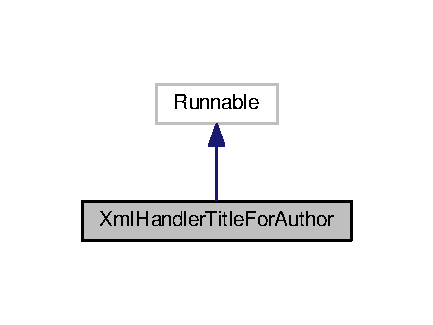
\includegraphics[width=208pt]{classXmlHandlerTitleForAuthor__inherit__graph}
\end{center}
\end{figure}


Collaboration diagram for Xml\-Handler\-Title\-For\-Author\-:
\nopagebreak
\begin{figure}[H]
\begin{center}
\leavevmode
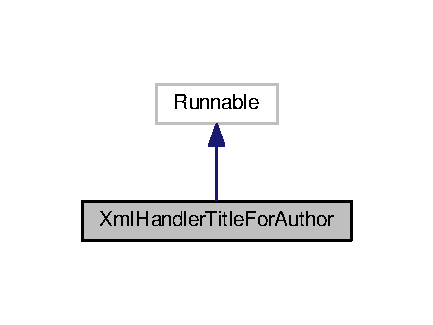
\includegraphics[width=208pt]{classXmlHandlerTitleForAuthor__coll__graph}
\end{center}
\end{figure}
\subsection*{Public Member Functions}
\begin{DoxyCompactItemize}
\item 
void \hyperlink{classXmlHandlerTitleForAuthor_af3adb501262a2822c56421f032877597}{fill\-File} ()
\item 
void \hyperlink{classXmlHandlerTitleForAuthor_ad366f324811314fadaf71266bab44d04}{sort} ()
\item 
void \hyperlink{classXmlHandlerTitleForAuthor_a97c8021ffd31638997b241891eb1c4ea}{set\-Author} (Array\-List$<$ String $>$ z)
\item 
void \hyperlink{classXmlHandlerTitleForAuthor_a8b6efd5dcc022fde5321b9ea8ba94215}{run} ()
\end{DoxyCompactItemize}
\subsection*{Public Attributes}
\begin{DoxyCompactItemize}
\item 
volatile int \hyperlink{classXmlHandlerTitleForAuthor_aacfb0b6097f6d67493b600563cc91ec7}{working}
\end{DoxyCompactItemize}


\subsection{Detailed Description}


Definition at line 8 of file Xml\-Handler\-Title\-For\-Author.\-java.



\subsection{Member Function Documentation}
\hypertarget{classXmlHandlerTitleForAuthor_af3adb501262a2822c56421f032877597}{\index{Xml\-Handler\-Title\-For\-Author@{Xml\-Handler\-Title\-For\-Author}!fill\-File@{fill\-File}}
\index{fill\-File@{fill\-File}!XmlHandlerTitleForAuthor@{Xml\-Handler\-Title\-For\-Author}}
\subsubsection[{fill\-File}]{\setlength{\rightskip}{0pt plus 5cm}void Xml\-Handler\-Title\-For\-Author.\-fill\-File (
\begin{DoxyParamCaption}
{}
\end{DoxyParamCaption}
)\hspace{0.3cm}{\ttfamily [inline]}}}\label{classXmlHandlerTitleForAuthor_af3adb501262a2822c56421f032877597}


Definition at line 13 of file Xml\-Handler\-Title\-For\-Author.\-java.


\begin{DoxyCode}
13                           \{
14         \textcolor{keywordflow}{try}\{
15             \hyperlink{classXmlHandlerTitleForAuthor_aacfb0b6097f6d67493b600563cc91ec7}{working} = 0;
16             System.setProperty(\textcolor{stringliteral}{"jdk.xml.entityExpansionLimit"}, \textcolor{stringliteral}{"0"});
17             PrintWriter write = \textcolor{keyword}{new} PrintWriter( \textcolor{keyword}{new} BufferedWriter( \textcolor{keyword}{new} FileWriter ( \textcolor{stringliteral}{"Ref.txt"}) ) );
18             write.close();
19             SAXParserFactory fac = SAXParserFactory.newInstance();
20             SAXParser saxTheFile = fac.newSAXParser();
21             DefaultHandler defHandler = \textcolor{keyword}{new} DefaultHandler()\{
22                 \textcolor{keywordtype}{int} counter = 0;
23                 String title,pages,url,volume,year,snum,journal;
24                 \textcolor{keywordtype}{boolean} titleCheck = \textcolor{keyword}{false},volCheck = \textcolor{keyword}{false},yearCheck = \textcolor{keyword}{false},urlCheck = \textcolor{keyword}{false},checkAuth = \textcolor{keyword}{
      false},pagesCheck = \textcolor{keyword}{false},checkforall = \textcolor{keyword}{false},journalCheck = \textcolor{keyword}{false},checkCat = \textcolor{keyword}{true};
25                 \textcolor{keyword}{public} \textcolor{keywordtype}{void} startElement(String uri,String localName,String qname,Attributes att)\textcolor{keywordflow}{throws} 
      SAXException\{
26                     \textcolor{keywordflow}{if}(qname.equals(\textcolor{stringliteral}{"www"}))\{
27                         checkCat = \textcolor{keyword}{false};
28                     \}
29                     \textcolor{keywordflow}{else} \textcolor{keywordflow}{if}(qname.equals(\textcolor{stringliteral}{"author"}))\{
30                         checkAuth = \textcolor{keyword}{true};
31                         join = \textcolor{stringliteral}{""};
32                     \}
33                     \textcolor{keywordflow}{else} \textcolor{keywordflow}{if}(qname.equals(\textcolor{stringliteral}{"title"}))\{
34                         titleCheck = \textcolor{keyword}{true};
35                     \}
36                     \textcolor{keywordflow}{else} \textcolor{keywordflow}{if}(qname.equals(\textcolor{stringliteral}{"year"}))\{
37                         yearCheck = \textcolor{keyword}{true};
38                     \}
39                     \textcolor{keywordflow}{else} \textcolor{keywordflow}{if}(qname.equals(\textcolor{stringliteral}{"url"}))\{
40                         urlCheck = \textcolor{keyword}{true};
41                     \}
42                     \textcolor{keywordflow}{else} \textcolor{keywordflow}{if}(qname.equals(\textcolor{stringliteral}{"pages"}))\{
43                         pagesCheck = \textcolor{keyword}{true};
44                     \}
45                     \textcolor{keywordflow}{else} \textcolor{keywordflow}{if}(qname.equals(\textcolor{stringliteral}{"volume"}))\{
46                         volCheck = \textcolor{keyword}{true};
47                     \}
48                     \textcolor{keywordflow}{else} \textcolor{keywordflow}{if}(qname.equals(\textcolor{stringliteral}{"journal"}) || qname.equals(\textcolor{stringliteral}{"booktitle"}))\{
49                         journalCheck = \textcolor{keyword}{true};
50                     \}
51                 \}
52                 \textcolor{keyword}{public} \textcolor{keywordtype}{void} characters(\textcolor{keywordtype}{char} chArray[],\textcolor{keywordtype}{int} start,\textcolor{keywordtype}{int} length)\textcolor{keywordflow}{throws} SAXException\{
53                     \textcolor{keywordflow}{if}(checkAuth && checkCat)\{
54                         String temp = \textcolor{keyword}{new} String(chArray,start,length); 
55                         join = join + temp;
56                         \textcolor{keywordflow}{for}(String x : auth)\{
57                             \textcolor{keywordflow}{if}(x.equalsIgnoreCase(join))\{
58                                 checkforall = \textcolor{keyword}{true};
59                             \}
60                         \}
61                     \}
62                     \textcolor{keywordflow}{else} \textcolor{keywordflow}{if}(titleCheck && checkCat && checkforall)\{
63                         title = \textcolor{keyword}{new} String(chArray,start,length);
64                     \}
65                     \textcolor{keywordflow}{else} \textcolor{keywordflow}{if}(volCheck && checkCat && checkforall)\{
66                         volume = \textcolor{keyword}{new} String(chArray,start,length);
67                     \}
68                     \textcolor{keywordflow}{else} \textcolor{keywordflow}{if}(pagesCheck && checkCat && checkforall)\{
69                         pages = \textcolor{keyword}{new} String(chArray,start,length);
70                     \}
71                     \textcolor{keywordflow}{else} \textcolor{keywordflow}{if}(urlCheck && checkCat && checkforall)\{
72                         url = \textcolor{keyword}{new} String(chArray,start,length);
73                     \}
74                     \textcolor{keywordflow}{else} \textcolor{keywordflow}{if}(yearCheck && checkCat && checkforall)\{
75                         year = \textcolor{keyword}{new} String(chArray,start,length);
76                     \}
77                     \textcolor{keywordflow}{else} \textcolor{keywordflow}{if}(journalCheck && checkCat && checkforall)\{
78                         journal = \textcolor{keyword}{new} String(chArray,start,length);
79                     \}
80                 \}
81                 \textcolor{keyword}{public} \textcolor{keywordtype}{void} endElement(String uri,String localName,String qname)\textcolor{keywordflow}{throws} SAXException\{
82                     \textcolor{keywordflow}{if}(qname.equals(\textcolor{stringliteral}{"title"}))\{
83                         titleCheck = \textcolor{keyword}{false};
84                     \}
85                     \textcolor{keywordflow}{else} \textcolor{keywordflow}{if}(qname.equals(\textcolor{stringliteral}{"url"}))\{
86                         urlCheck = \textcolor{keyword}{false};
87                         \textcolor{keywordflow}{if}(!checkforall)\{
88                             author.clear();
89                         \}
90                         \textcolor{keywordflow}{else}\{
91                             counter = counter + 1;
92                             snum = Integer.toString(counter);
93                             writer(snum,author,title,url,year,pages,volume,journal);
94                             checkforall = \textcolor{keyword}{false};                
95                         \}
96                     \}
97                     \textcolor{keywordflow}{else} \textcolor{keywordflow}{if}(qname.equals(\textcolor{stringliteral}{"year"}))\{
98                         yearCheck = \textcolor{keyword}{false};
99                     \}
100                     \textcolor{keywordflow}{else} \textcolor{keywordflow}{if}(qname.equals(\textcolor{stringliteral}{"pages"}))\{
101                         pagesCheck = \textcolor{keyword}{false};
102                     \}
103                     \textcolor{keywordflow}{else} \textcolor{keywordflow}{if}(qname.equals(\textcolor{stringliteral}{"volume"}))\{
104                         volCheck = \textcolor{keyword}{false};
105                     \}
106                     \textcolor{keywordflow}{else} \textcolor{keywordflow}{if}(qname.equals(\textcolor{stringliteral}{"journal"}) || qname.equals(\textcolor{stringliteral}{"booktitle"}))\{
107                         journalCheck = \textcolor{keyword}{false};
108                     \}
109                     \textcolor{keywordflow}{else} \textcolor{keywordflow}{if}(qname.equals(\textcolor{stringliteral}{"author"}))\{
110                         checkAuth = \textcolor{keyword}{false};
111                         author.add(join);
112                     \}
113                 \}
114             \};
115             saxTheFile.parse(\textcolor{stringliteral}{"dblp.xml"},defHandler);
116         \}
117         \textcolor{keywordflow}{catch}(Exception e)\{
118             e.printStackTrace();
119         \}
120     \}
\end{DoxyCode}
\hypertarget{classXmlHandlerTitleForAuthor_a8b6efd5dcc022fde5321b9ea8ba94215}{\index{Xml\-Handler\-Title\-For\-Author@{Xml\-Handler\-Title\-For\-Author}!run@{run}}
\index{run@{run}!XmlHandlerTitleForAuthor@{Xml\-Handler\-Title\-For\-Author}}
\subsubsection[{run}]{\setlength{\rightskip}{0pt plus 5cm}void Xml\-Handler\-Title\-For\-Author.\-run (
\begin{DoxyParamCaption}
{}
\end{DoxyParamCaption}
)\hspace{0.3cm}{\ttfamily [inline]}}}\label{classXmlHandlerTitleForAuthor_a8b6efd5dcc022fde5321b9ea8ba94215}


Definition at line 177 of file Xml\-Handler\-Title\-For\-Author.\-java.


\begin{DoxyCode}
177                   \{
178     \hyperlink{classXmlHandlerTitleForAuthor_af3adb501262a2822c56421f032877597}{fillFile}();
179     \hyperlink{classXmlHandlerTitleForAuthor_ad366f324811314fadaf71266bab44d04}{sort}();
180 \}
\end{DoxyCode}
\hypertarget{classXmlHandlerTitleForAuthor_a97c8021ffd31638997b241891eb1c4ea}{\index{Xml\-Handler\-Title\-For\-Author@{Xml\-Handler\-Title\-For\-Author}!set\-Author@{set\-Author}}
\index{set\-Author@{set\-Author}!XmlHandlerTitleForAuthor@{Xml\-Handler\-Title\-For\-Author}}
\subsubsection[{set\-Author}]{\setlength{\rightskip}{0pt plus 5cm}void Xml\-Handler\-Title\-For\-Author.\-set\-Author (
\begin{DoxyParamCaption}
\item[{Array\-List$<$ String $>$}]{z}
\end{DoxyParamCaption}
)\hspace{0.3cm}{\ttfamily [inline]}}}\label{classXmlHandlerTitleForAuthor_a97c8021ffd31638997b241891eb1c4ea}


Definition at line 173 of file Xml\-Handler\-Title\-For\-Author.\-java.


\begin{DoxyCode}
173                                           \{
174     auth = z;
175 \}
\end{DoxyCode}
\hypertarget{classXmlHandlerTitleForAuthor_ad366f324811314fadaf71266bab44d04}{\index{Xml\-Handler\-Title\-For\-Author@{Xml\-Handler\-Title\-For\-Author}!sort@{sort}}
\index{sort@{sort}!XmlHandlerTitleForAuthor@{Xml\-Handler\-Title\-For\-Author}}
\subsubsection[{sort}]{\setlength{\rightskip}{0pt plus 5cm}void Xml\-Handler\-Title\-For\-Author.\-sort (
\begin{DoxyParamCaption}
{}
\end{DoxyParamCaption}
)\hspace{0.3cm}{\ttfamily [inline]}}}\label{classXmlHandlerTitleForAuthor_ad366f324811314fadaf71266bab44d04}


Definition at line 138 of file Xml\-Handler\-Title\-For\-Author.\-java.


\begin{DoxyCode}
138                       \{
139         \textcolor{keywordflow}{try}\{
140             List<ArrayList<String>> csvLines = \textcolor{keyword}{new} ArrayList<ArrayList<String>>();
141             Comparator<ArrayList<String>> comp = \textcolor{keyword}{new} Comparator<ArrayList<String>>() \{
142                 \textcolor{keyword}{public} \textcolor{keywordtype}{int} compare(ArrayList<String> csvLine1, ArrayList<String> csvLine2) \{
143                     \textcolor{keywordtype}{int} x = Integer.valueOf(csvLine1.get(4)).compareTo(Integer.valueOf(csvLine2.get(4)));
144                     \textcolor{keywordflow}{return} -x;
145                 \}
146             \};
147             BufferedReader read = \textcolor{keyword}{new} BufferedReader(\textcolor{keyword}{new} FileReader(\textcolor{stringliteral}{"Ref.txt"}));
148             String call;
149             \textcolor{keywordflow}{while}((call = read.readLine())!= null)\{
150             ArrayList<String> temp = \textcolor{keyword}{new} ArrayList<String>();
151             String[] x = call.split(\textcolor{stringliteral}{"~"});
152             \textcolor{keywordflow}{for}(\textcolor{keywordtype}{int} i = 0;i<x.length;i++)\{
153                 temp.add(x[i]);
154             \}
155             csvLines.add(temp);
156             \}
157             read.close();
158             Collections.sort(csvLines,comp);
159             PrintWriter write = \textcolor{keyword}{new} PrintWriter( \textcolor{keyword}{new} BufferedWriter( \textcolor{keyword}{new} FileWriter ( \textcolor{stringliteral}{"Ref.txt"}) ) );
160             \textcolor{keywordflow}{for}(\textcolor{keywordtype}{int} i = 0;i<csvLines.size();i++)\{
161                 write.print((i+1)+\textcolor{stringliteral}{"~"}+csvLines.get(i).get(1)+ \textcolor{stringliteral}{"~"} +csvLines.get(i).get(2)+ \textcolor{stringliteral}{"~"} +csvLines.
      get(i).get(3)+ \textcolor{stringliteral}{"~"} + csvLines.get(i).get(4) + \textcolor{stringliteral}{"~"}+ csvLines.get(i).get(5)+ \textcolor{stringliteral}{"~"} + csvLines.get(i).get(6)+ \textcolor{stringliteral}{"~"} +
       csvLines.get(i).get(7) +\textcolor{stringliteral}{"\(\backslash\)n"});
162                 write.flush();
163             \}
164             write.close();
165         \}   \textcolor{keywordflow}{catch}(Exception e)
166         \{
167             e.printStackTrace();
168         \}
169         \textcolor{keywordflow}{finally}\{
170             \hyperlink{classXmlHandlerTitleForAuthor_aacfb0b6097f6d67493b600563cc91ec7}{working} = 1;
171         \}
172         \}
\end{DoxyCode}


\subsection{Member Data Documentation}
\hypertarget{classXmlHandlerTitleForAuthor_aacfb0b6097f6d67493b600563cc91ec7}{\index{Xml\-Handler\-Title\-For\-Author@{Xml\-Handler\-Title\-For\-Author}!working@{working}}
\index{working@{working}!XmlHandlerTitleForAuthor@{Xml\-Handler\-Title\-For\-Author}}
\subsubsection[{working}]{\setlength{\rightskip}{0pt plus 5cm}volatile int Xml\-Handler\-Title\-For\-Author.\-working}}\label{classXmlHandlerTitleForAuthor_aacfb0b6097f6d67493b600563cc91ec7}


Definition at line 11 of file Xml\-Handler\-Title\-For\-Author.\-java.



The documentation for this class was generated from the following file\-:\begin{DoxyCompactItemize}
\item 
\hyperlink{XmlHandlerTitleForAuthor_8java}{Xml\-Handler\-Title\-For\-Author.\-java}\end{DoxyCompactItemize}

\chapter{File Documentation}
\hypertarget{Loading_8java}{\section{Loading.\-java File Reference}
\label{Loading_8java}\index{Loading.\-java@{Loading.\-java}}
}
\subsection*{Classes}
\begin{DoxyCompactItemize}
\item 
class \hyperlink{classLoading}{Loading}
\end{DoxyCompactItemize}

\hypertarget{Query1__GUI_8java}{\section{Query1\-\_\-\-G\-U\-I.\-java File Reference}
\label{Query1__GUI_8java}\index{Query1\-\_\-\-G\-U\-I.\-java@{Query1\-\_\-\-G\-U\-I.\-java}}
}
\subsection*{Classes}
\begin{DoxyCompactItemize}
\item 
class \hyperlink{classQuery1__GUI}{Query1\-\_\-\-G\-U\-I}
\end{DoxyCompactItemize}

\hypertarget{Query2__GUI_8java}{\section{Query2\-\_\-\-G\-U\-I.\-java File Reference}
\label{Query2__GUI_8java}\index{Query2\-\_\-\-G\-U\-I.\-java@{Query2\-\_\-\-G\-U\-I.\-java}}
}
\subsection*{Classes}
\begin{DoxyCompactItemize}
\item 
class \hyperlink{classQuery2__GUI}{Query2\-\_\-\-G\-U\-I}
\end{DoxyCompactItemize}

\hypertarget{Query3__GUI_8java}{\section{Query3\-\_\-\-G\-U\-I.\-java File Reference}
\label{Query3__GUI_8java}\index{Query3\-\_\-\-G\-U\-I.\-java@{Query3\-\_\-\-G\-U\-I.\-java}}
}
\subsection*{Classes}
\begin{DoxyCompactItemize}
\item 
class \hyperlink{classQuery3__GUI}{Query3\-\_\-\-G\-U\-I}
\end{DoxyCompactItemize}

\hypertarget{Search_8java}{\section{Search.\-java File Reference}
\label{Search_8java}\index{Search.\-java@{Search.\-java}}
}
\subsection*{Classes}
\begin{DoxyCompactItemize}
\item 
class \hyperlink{classSearch}{Search}
\end{DoxyCompactItemize}

\hypertarget{XmlHandler_8java}{\section{Xml\-Handler.\-java File Reference}
\label{XmlHandler_8java}\index{Xml\-Handler.\-java@{Xml\-Handler.\-java}}
}
\subsection*{Classes}
\begin{DoxyCompactItemize}
\item 
class \hyperlink{classXmlHandlerAuthor}{Xml\-Handler\-Author}
\end{DoxyCompactItemize}

\hypertarget{XmlHandlerAuthor_8java}{\section{Xml\-Handler\-Author.\-java File Reference}
\label{XmlHandlerAuthor_8java}\index{Xml\-Handler\-Author.\-java@{Xml\-Handler\-Author.\-java}}
}
\subsection*{Classes}
\begin{DoxyCompactItemize}
\item 
class \hyperlink{classXmlHandlerAuthor}{Xml\-Handler\-Author}
\end{DoxyCompactItemize}

\hypertarget{XmlHandlerTitle_8java}{\section{Xml\-Handler\-Title.\-java File Reference}
\label{XmlHandlerTitle_8java}\index{Xml\-Handler\-Title.\-java@{Xml\-Handler\-Title.\-java}}
}
\subsection*{Classes}
\begin{DoxyCompactItemize}
\item 
class \hyperlink{classXmlHandlerTitle}{Xml\-Handler\-Title}
\end{DoxyCompactItemize}

\hypertarget{XmlHandlerTitleForAuthor_8java}{\section{Xml\-Handler\-Title\-For\-Author.\-java File Reference}
\label{XmlHandlerTitleForAuthor_8java}\index{Xml\-Handler\-Title\-For\-Author.\-java@{Xml\-Handler\-Title\-For\-Author.\-java}}
}
\subsection*{Classes}
\begin{DoxyCompactItemize}
\item 
class \hyperlink{classXmlHandlerTitleForAuthor}{Xml\-Handler\-Title\-For\-Author}
\end{DoxyCompactItemize}

%--- End generated contents ---

% Index
\newpage
\phantomsection
\addcontentsline{toc}{chapter}{Index}
\printindex

\end{document}
